%%%%%%%%%%%%%%%%%%%%%%%%%%%%%%%%%%%%%%%%%%%%%%%%%%%%%%%%%%%%%%%%%%%%%%%%%%%%%%%%%%%%%%%%%%%%%%%%%%%%%%%%%%%%%%%%%%%%%%%%%%%%%%%%%%%%%%%%%%%%%%%%%%%%%%%%%%%
% This is just an example/guide for you to refer to when submitting manuscripts to Frontiers, it is not mandatory to use Frontiers .cls files nor frontiers.tex  %
% This will only generate the Manuscript, the final article will be typeset by Frontiers after acceptance.
%                                              %
%                                                                                                                                                         %
% When submitting your files, remember to upload this *tex file, the pdf generated with it, the *bib file (if bibliography is not within the *tex) and all the figures.
%%%%%%%%%%%%%%%%%%%%%%%%%%%%%%%%%%%%%%%%%%%%%%%%%%%%%%%%%%%%%%%%%%%%%%%%%%%%%%%%%%%%%%%%%%%%%%%%%%%%%%%%%%%%%%%%%%%%%%%%%%%%%%%%%%%%%%%%%%%%%%%%%%%%%%%%%%%

%%% Version 3.4 Generated 2018/06/15 %%%
%%% You will need to have the following packages installed: datetime, fmtcount, etoolbox, fcprefix, which are normally inlcuded in WinEdt. %%%
%%% In http://www.ctan.org/ you can find the packages and how to install them, if necessary. %%%
%%%  NB logo1.jpg is required in the path in order to correctly compile front page header %%%

\documentclass[utf8]{frontiersSCNS} % for Science, Engineering and Humanities and Social Sciences articles
%\documentclass[utf8]{frontiersHLTH} % for Health articles
%\documentclass[utf8]{frontiersFPHY} % for Physics and Applied Mathematics and Statistics articles

%\setcitestyle{square} % for Physics and Applied Mathematics and Statistics articles
\usepackage{url,hyperref,lineno,microtype,subcaption}
\usepackage[onehalfspacing]{setspace}
\graphicspath{ {./plots/} }

% \linenumbers


% Leave a blank line between paragraphs instead of using \\


\def\keyFont{\fontsize{8}{11}\helveticabold }
\def\firstAuthorLast{Ozturk {et~al.}} %use et al only if is more than 1 author
\def\Authors{Abdurrahman Ozturk\,$^{1,*}$, Merve Gencturk\,$^{1}$, Karim Ahmed\,$^{1}$}
% Affiliations should be keyed to the author's name with superscript numbers and be listed as follows: Laboratory, Institute, Department, Organization, City, State abbreviation (USA, Canada, Australia), and Country (without detailed address information such as city zip codes or street names).
% If one of the authors has a change of address, list the new address below the correspondence details using a superscript symbol and use the same symbol to indicate the author in the author list.
\def\Address{$^{1}$Department of Nuclear Engineering, Texas A\&M University, USA}
% The Corresponding Author should be marked with an asterisk
% Provide the exact contact address (this time including street name and city zip code) and email of the corresponding author
\def\corrAuthor{Abdurrahman Ozturk}
\def\corrEmail{aozturk@tamu.edu}




\begin{document}
\onecolumn
\firstpage{1}

\title[Numerical Solution of Rate Theory Equations]{Numerical Solution of Point Defect(Rate Theory) Equations (in MOOSE)}

\author[\firstAuthorLast ]{\Authors} %This field will be automatically populated
\address{} %This field will be automatically populated
\correspondance{} %This field will be automatically populated

\extraAuth{}% If there are more than 1 corresponding author, comment this line and uncomment the next one.
%\extraAuth{corresponding Author2 \\ Laboratory X2, Institute X2, Department X2, Organization X2, Street X2, City X2 , State XX2 (only USA, Canada and Australia), Zip Code2, X2 Country X2, email2@uni2.edu}


\maketitle


\begin{abstract}

%%% Leave the Abstract empty if your article does not require one, please see the Summary Table for full details.
\section{}
We present a detailed investigation of the effect of size on the segregation of point defects to interfaces and the resultant nucleation of voids. We utilize the spatially-resolved rate-theory (SRRT) modeling technique valid for modeling surfaces as discrete sinks. The effects of defect production rate, bias, and profile are thoroughly studied. The model predictions are generally different from the textbook ones obtained by the classical homogenized rate theory approach. The simulations show a strong dependence of the steady state defect profiles on the grain size, temperature, and production rate, bias, and profile. Moreover, the sink strength of each boundary is also affected by these factors. Furthermore, it is predicted that whenever there is a production bias, no neutral sinks can exist, i.e., there is always a preference for surfaces/interfaces to absorb one type of defects over another. The model predictions demonstrate the shortcomings of the classical homogeneous rate-theory approach and shed light on the limitations of using ion irradiation to mimic neutron irradiation.

\tiny
 \keyFont{ \section{Keywords:} point defect equations, rate theory, interstitial, vacancy, radiation damage, MOOSE} %All article types: you may provide up to 8 keywords; at least 5 are mandatory.
\end{abstract}

\section{Introduction}

\textcolor{red}{
-articles about neutron, proton, ion irradiation\\
radiation damage/interactions//
motivation about paper//
Harsh conditions//
neutron-ion case comparison//
instabilities, extended defects (Ghoniem paper)//
in this study, focusing effect of grain size, bias, discrete surfaces,
homogenized RT, spatially resolution//
qualifying extended defects//
profiles change with increasing radiation damage
}
% For Original Research Articles \citep{conference}, Clinical Trial Articles \citep{article}, and Technology Reports \citep{patent}, the introduction should be succinct, with no subheadings \citep{book}. For Case Reports the Introduction should include symptoms at presentation \citep{chapter}, physical exams and lab results \citep{dataset}.

\section{Methodology}

% For requirements for a specific article type please refer to the Article Types on any Frontiers journal page. Please also refer to  \href{http://home.frontiersin.org/about/author-guidelines#Sections}{Author Guidelines} for further information on how to organize your manuscript in the required sections or their equivalents for your field

% For Original Research articles, please note that the Material and Methods section can be placed in any of the following ways: before Results, before Discussion or after Discussion.

\subsection{Point Defect Equations}
    The irradiation of a material causes the creation of vacancies and interstitial because of atomic collisions. The point defects can diffuse through material, recombine with each other, and react with sinks which are present in microstructure. The concentration of point defects is described mathematically by the chemical rate balance equations given in following sets of equations.

\begin{equation}
  \begin{aligned}
    &\frac{dC_i}{dt} = K_0 - K_{iv}C_iC_v - K_{is}C_iC_s + \nabla\cdot D_i\nabla C_i\\
    &\frac{dC_v}{dt} = (1+b)K_0 - K_{iv}C_iC_v - K_{vs}C_vC_s + \nabla\cdot D_v\nabla C_v
  \end{aligned}
  \label{equation:point_defect_equations}
\end{equation}

    There are different terms with different rate coefficients as seen in Eq. \ref{equation:point_defect_equations}. The first term on the RHS is a source term, representing defect generation with rate of \textit{K\textsubscript{0}}. In vacancy equation, \textit{b} is used as percent production bias to create a difference between interstitial and vacancy generation in domain. The second term is a reaction term, referring the recombination process if the defect \textit{x} reacts with defect \textit{y} with a rate of \textit{K\textsubscript{xy}}. The third term is also a reaction term, representing the reaction between the defect \textit{x} and the sink \textit{s} with a rate of \textit{K\textsubscript{xs}}. In this study, the sink concentration is assumed constant and uniformly distributed over domain. The last term is diffusion term which is resolving the spatial behavior of defects.\\
    Another form of point defect equations can be written by using sink strength, \textit{k} definition for sink reaction term.

\begin{equation}
  \begin{aligned}
    &k_i^2D_iC_i = K_{is}C_iC_s \\
    &k_v^2D_vC_v = K_{vs}C_vC_s \\
  \end{aligned}
  \label{equation:sink_reaction_term}
\end{equation}\\
\begin{equation}
  \begin{aligned}
    &\frac{dC_i}{dt} = K_0 - K_{iv}C_iC_v - k_i^2D_iC_i + \nabla\cdot D_i\nabla C_i\\
    &\frac{dC_v}{dt} = (1+b)K_0 - K_{iv}C_iC_v - k_v^2D_vC_v + \nabla\cdot D_v\nabla C_v\\
  \end{aligned}
  \label{equation:point_defect_equations_sink_strength}
\end{equation}\\

\subsection{Non-dimensionalization of Point Defect Equations}
    The time space of defect interactions is enormously large, which could differ from nanoseconds to hours. Additionally, reaction rate coefficients also have different orders of magnitude. To deal with inconsistent dimensions, non-dimensionalized form of equations can be considered for numerical solution. To that end, the following non-dimensionalization scheme and scaling factors are introduced.

    \begin{equation}
      \begin{aligned}
        &X = \Omega C\\
        &\tau = \frac{t}{\omega}\\
      \end{aligned}
      \label{equation:non-dimensionalization_variables}
    \end{equation}

    where ${\Omega}$ is atomic volume in ${m^3}$, ${l}$ is length scale in ${m}$ and ${\omega}$ is time scale in ${s}$, ${\omega= l^2/D_i}$\\

    After substituting Eq. \ref{equation:non-dimensionalization_variables} into \ref{equation:point_defect_equations} and reorganizing, final form  of non-dimensionalized point defect equations become,

    \begin{equation}
      \begin{aligned}
        &\frac{dX_i}{dt} = \Omega\omega K_0 - \frac{\omega K_{iv}}{\Omega}X_iX_v - \frac{\omega K_{is}}{\Omega}X_iX_s + \omega D_i\nabla^2 X_i\\
        &\frac{dX_v}{dt} = \Omega\omega K_0 - \frac{\omega K_{iv}}{\Omega}X_iX_v - \frac{\omega K_{vs}}{\Omega}X_vX_s + \omega D_v\nabla^2 X_v\\
      \end{aligned}
      \label{equation:non-dimensionalized_point_defect_equations}
    \end{equation}\\
    or
    \begin{equation}
      \begin{aligned}
        &\frac{dX_i}{dt} = \widetilde{K_0} - \widetilde{K_{iv}}X_iX_v - \widetilde{K_{is}}X_iX_s + \widetilde{D_i}\widetilde{\nabla}^2 X_i\\
        &\frac{dX_v}{dt} = \widetilde{K_0} - \widetilde{K_{iv}}X_iX_v - \widetilde{K_{vs}}X_vX_s + \widetilde{D_v}\widetilde{\nabla}^2 X_v\\
      \end{aligned}
      \label{equation:non-dimensionalized_point_defect_equations}
    \end{equation}

    The Multiphysics Object-Oriented Simulation Environment (MOOSE) is used as tool to solve point defect equations numerically. MOOSE is an open-source framework that provides users to solve partial differential equations (PDEs) and build a state-of-the-art, computationally scalable finite element-based simulations. \textcolor{red}{ref.}\\

\subsection{Model Settings and Parameters}
    Ni-based alloys have been used in many nuclear reactors applications because of their excellent corrosion resistance and high mechanical properties. For example, Ni-based alloys containing 15-30\% Cr are generally used in reactor cooling systems due to their corrosion resistance. However, their properties change under irradiation and needs to be investigated. \textcolor{red}{irradiation induced embrittlement, phase instability, and swelling. It is essential to predict the material structure changes due to radiation accurately.} \citep{walgraef1996}

    \textcolor{blue}{
    Nickel is selected as base material for this study, and its properties; lattice parameter, $a$, is 0.352 $nm$, atomic volume, $V$, is 0.01206 $nm^3$, migration energy for interstitial, $E_{m,i}$, is 0.30 $eV$, migration energy for vacancy, $E_{m,v}$, is 1.30 $eV$, formation energy for interstitial, $E_{f,i}$, is 4.27 $eV$, formation energy for vacancy, $E_{f,v}$, is 1.60 $eV$, diffusion coefficient for interstitial, $D_{0,i}$, is 1e-7 $m^2/s$, and diffusion coefficient for vacancy, $D_{0,v}$, is 6e-5 $m^2/s$.
    \citep{ref}
    }\\

    \textcolor{blue}{
    In this study, three different irradiation types, neutrons, protons and ions, are considered. Their simulations are categorized into two groups based on defect production profile; uniform and non-uniform defect production. Neutrons are highly penetrable and causes uniform defect production on target material. Protons are not able to penetrate as much as neutrons do, but for small domain sizes, their defect production can be assumed as uniform. Ions or heavy charged particles loose their energies quickly and cause a non-uniform defect production. Table \ref{table:simulation_parameters} shows simulation parameters and values.
    }
    \begin{table}[h!]
      \caption{Simulation Parameters}
      \label{table:simulation_parameters}
      \begin{tabular}{ ||>{\centering\arraybackslash}p{3.5cm}|>{\centering\arraybackslash}p{2cm}|>{\centering\arraybackslash}p{3cm}|>{\centering\arraybackslash}p{3cm}|>{\centering\arraybackslash}p{3.5cm}||  }
         % \multicolumn{5}{|c|}{Simulation Parameters} \\
         \hline
         Defect Production & Type & Dose Rate (dpa/s) & Temperature (K) & Sink Density (m^{-3})\\
         \hline
         \hline
         Uniform     & Neutron  & 1e-6  & 773 & 1e18\\
                     & Proton   & 1e-3  & 773 & 1e18\\
         \hline
         Non-Uniform & Ion      & 1e-3  & 773 & 1e18\\
         % Distributed &           & 1e-6  & 773 & 1e18\\
         \hline
      \end{tabular}
    \end{table}

% \textcolor{red}{
% Hoca, bu type neutron,ion kısım için neutron case de high dose rate için proton diyerek ekleyebiliriz bu kısmı tartışalım dedi. Apo'nun yazdığı kısmı etkileyecek hocam apo ile beraber tekrar tartışalım dedim. Bu kısmı sorarız tekrar.
% }

% \textcolor{red}{
% Tables should be inserted at the end of the manuscript. Please build your table directly in LaTeX.Tables provided as jpeg/tiff files will not be accepted. Please note that very large tables (covering several pages) cannot be included in the final PDF for reasons of space. These tables will be published as \href{http://home.frontiersin.org/about/author-guidelines#SupplementaryMaterial}{Supplementary Material} on the online article page at the time of acceptance. The author will be notified during the typesetting of the final article if this is the case.
% }

\section{Results}

    Regarding cost and time, it can be understood that ion radiation has been used for a long time in experimental studies. However, with the development of reactor designs and the increase of long-term licensed reactors, it has been necessary to search for more reliable materials that can operate for a long time under extreme conditions. Therefore, it is essential to investigate the effects of neutron irradiation and ion irradiation in microstructure to determine the equality of neutron and ion irradiation results.

    The results obtained from MOOSE simulations are presented in this section by plots of defect concentration, vacancy supersaturation and sink strengths. The equations are solved in one direction using Lagrange elements and a second-order time integration scheme. In this work, the surfaces represent free surfaces or grain boundaries.\\ %The calculated sink strengths are also tabulated for different grain size and bias rates.

\subsection{Uniform Irradiation}
    Neutrons have an energy spectrum that varies a couple of orders of magnitude. This makes defect generation possible at different energies. Also, the high penetration depth of neutrons allow them to travel through material corresponding to their energies. Thus, they cause a uniform or flat-like defect production profile in material. \citep{was2017}

    Numerical models are frequently used to solve scientific problems and make decisions based on results obtained from simulations, but first, the numerical approach should be reliable. Before presenting results from this study, a simple spherical grain problem for neutron irradiation is solved by MOOSE as benchmark problem, and its results are compared to analytical results for validation.

    In this approach, unlike the simulations in this study, the mutual recombination term in Eq. \ref{equation:point_defect_equations_sink_strength} is neglected, and the steady state analytical solutions for a spherical grain of radius \textit{a} are found as below. \citep{heald1977}\\

    \begin{equation}
        \begin{aligned}
          &0 = \frac{K_0}{D_i} - k_i^2C_i + \frac{d^2C_i}{dr^2}+\frac{2}{r}\frac{dC_i}{dr}\\
          &0 = \frac{K_0}{D_v} - k_v^2C_v + \frac{d^2C_v}{dr^2}+\frac{2}{r}\frac{dC_v}{dr}\\
        \end{aligned}
        \label{equation:spherical_norecomb_point_defect_equations}
    \end{equation}\\

    \begin{equation}
        \begin{aligned}
          &C_i(r)=\frac{K_0}{D_ik_i^2}\bigg(1-\frac{a\sinh{k_ir}}{r\sinh{k_ia}}\bigg)\\
          &C_v(r)=\frac{K_0}{D_vk_v^2}\bigg(1-\frac{a\sinh{k_vr}}{r\sinh{k_va}}\bigg)\\
        \end{aligned}
        \label{equation:spherical_grain_analytical_solution}
    \end{equation}\\

    This approach is tested in MOOSE by solving point defect concentrations for a spherical grain having radius of 500 nm. As seen in Fig. \ref{figure:concentrations_MOOSE_analytical}, MOOSE results exactly match with the analytical solution, which makes it a useful tool to analyze behavior of defect concentrations.\\

    \begin{figure}[h!]
        \centering
        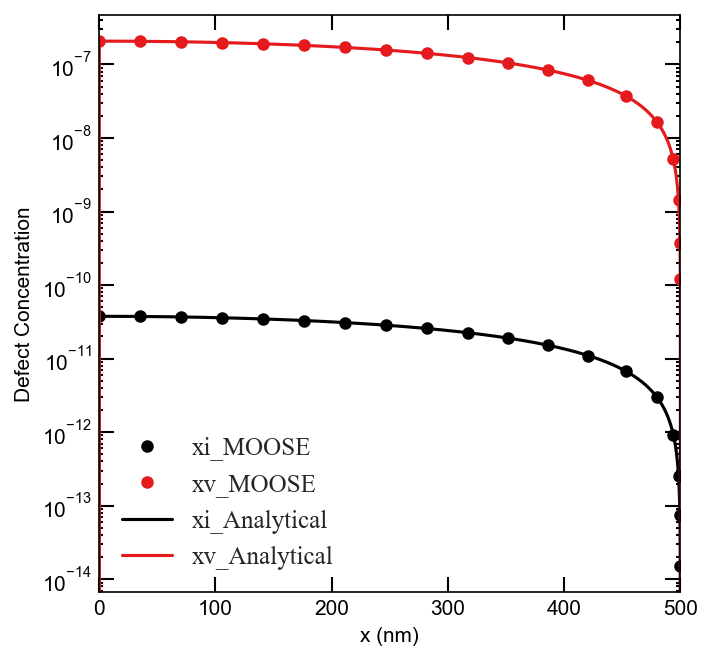
\includegraphics[scale=0.55]{concentration_profiles_MOOSE_Analytical_Neutron_0}
        \caption{Comparison of MOOSE results with analytical solution for spherical grain (\textit{a}=500 nm).}
        \label{figure:concentrations_MOOSE_analytical}
    \end{figure}

 \subsubsection{Concentrations}
    The defect concentrations can follow different patterns depending on their properties. Interstitials diffuse to sinks faster than vacancies, so their steady-state concentrations become lower (see Fig. \ref{figure:average_concentrations_neutron_5}). The effect of grain size and dose rate are shown in the same figure. The effect of grain size on the point defect kinetics resembles to some extent the effect of temperature. This is due to the fact that both factors affect the diffusion kinetics of defects. However, as will be discussed shortly, its effect on the steady-state spatial profiles is even more complicated. The dose rate acts as an amplifier and changes the intensity of the defect behavior. Thus the separation between defect concentrations becomes more explicit.

\textcolor{red}{
instability (flipping) affects the steady state concentrations levels//
abnormal concentration behaviors for both transient(proposed in papers) steady state(observed in this study)//
with grain size increase, defect concentrations diverges. this might initiate problems for physical properties, mechanical properties//
less recombination, more vacancy more void more swelling
}

    \begin{figure}[h!]  %Neutron - average conc - %5 Bias rate
        \centering
        a)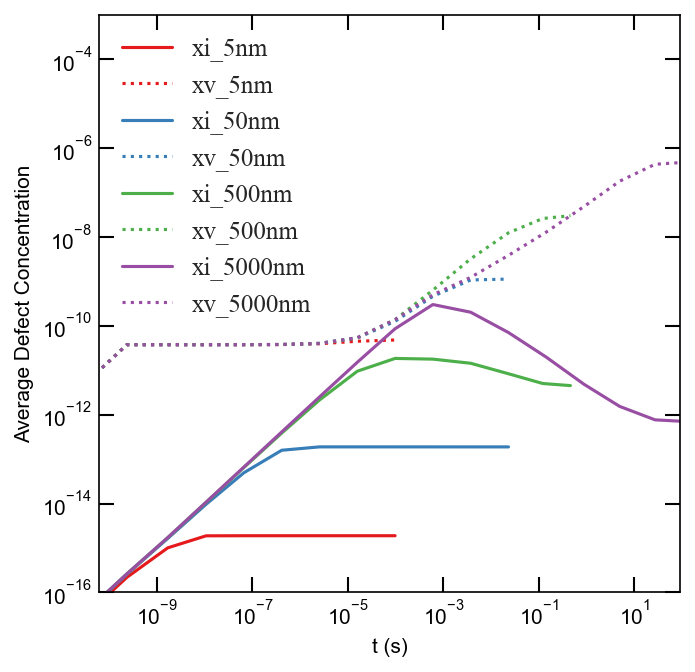
\includegraphics[scale=0.55]{average_concentration_neutron_5_size}
        \qquad
        b)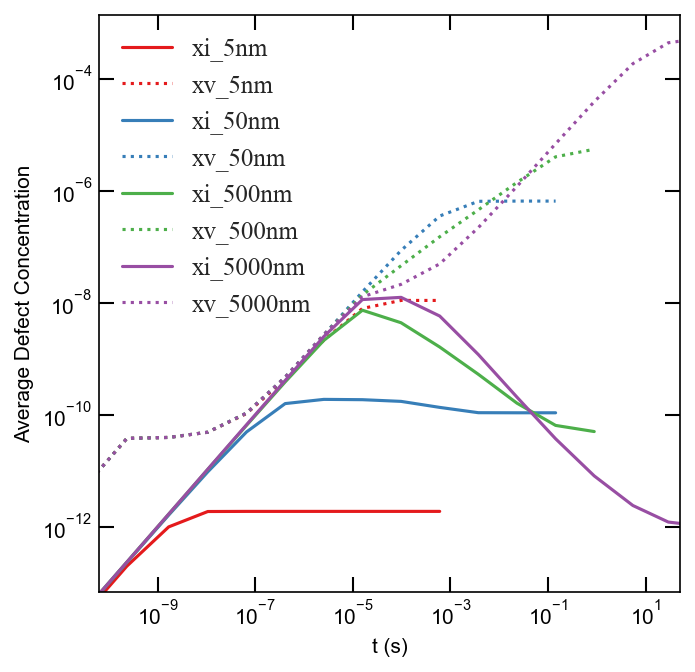
\includegraphics[scale=0.55]{average_concentration_high_neutron_5_size}
        \caption{Time-dependent behavior of average defect concentration for different grain sizes with 5\% production bias for a) neutrons and b) protons}
        \label{figure:average_concentrations_neutron_5}
    \end{figure}

    Atomic collisions create vacancy-interstitial pairs, but following events cause a vacancy dense defect population. This situation must be considered to make simulations physically more accurate. Production bias is used to ensure this imbalance in modeling point defects. The equal defect production, unbiased condition, is also studied for comparison.

    Uniform defect production and equilibrium condition at boundaries result in a symmetrical concentration profile around the domain center for neutron case. The steady-state concentrations at the center doesn't change significantly with increasing size, as shown in Fig. \ref{figure:concentrations_neutron_0_1e-6}.

    Protons tend to create more defect on material, and consequently concentration levels are higher compared to neutrons.(see Fig. \ref{figure:concentrations_neutron_0_1e-3}).

    % \begin{figure}[h!]  %Neutron - 1e-6 dpa/s - %0 Bias rate
    %     \centering
    %     a)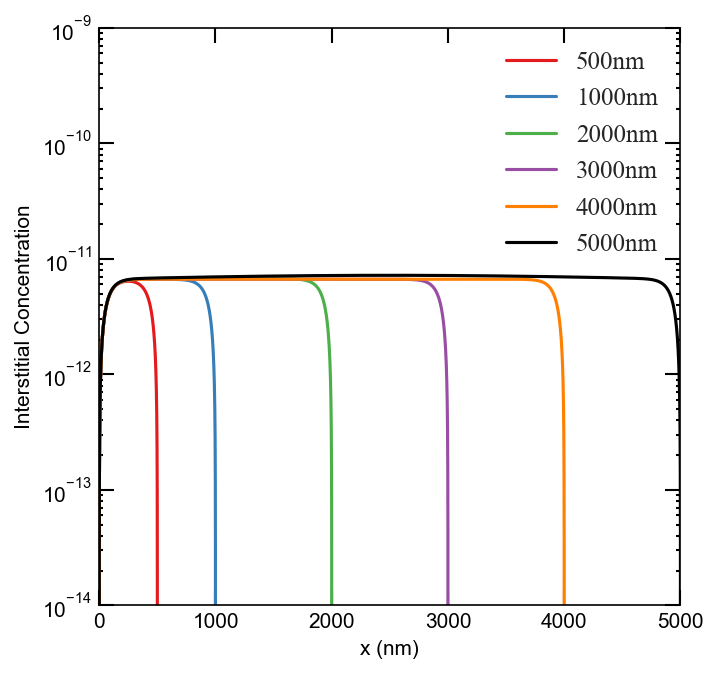
\includegraphics[scale=0.55]{interstitial_concentration_500-5000nm-neutron-0}
    %     b)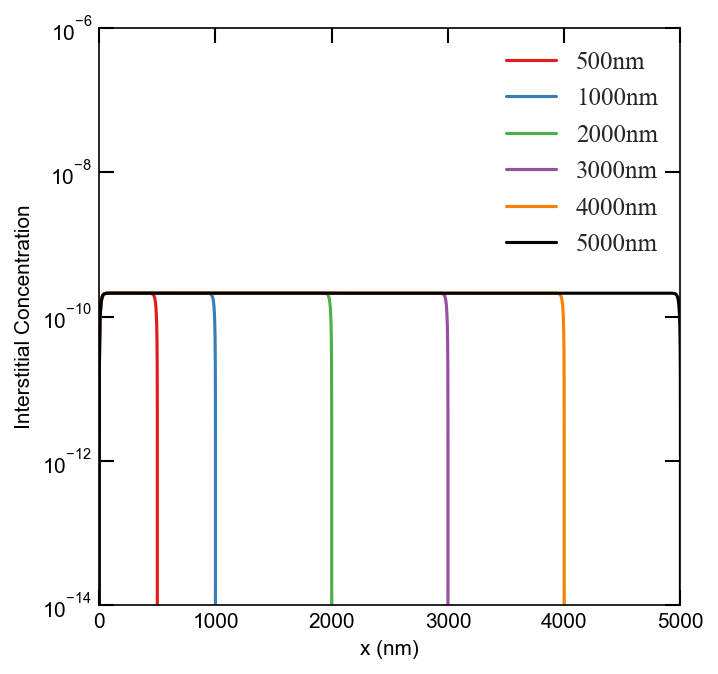
\includegraphics[scale=0.55]{interstitial_concentration_500-5000nm-high_neutron-0}
    %     c)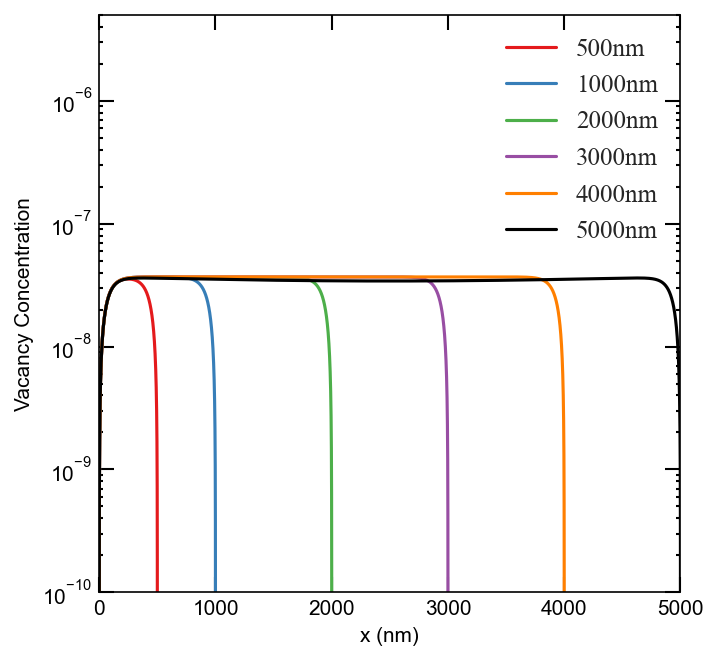
\includegraphics[scale=0.55]{vacancy_concentration_500-5000nm-neutron-0}
    %     d)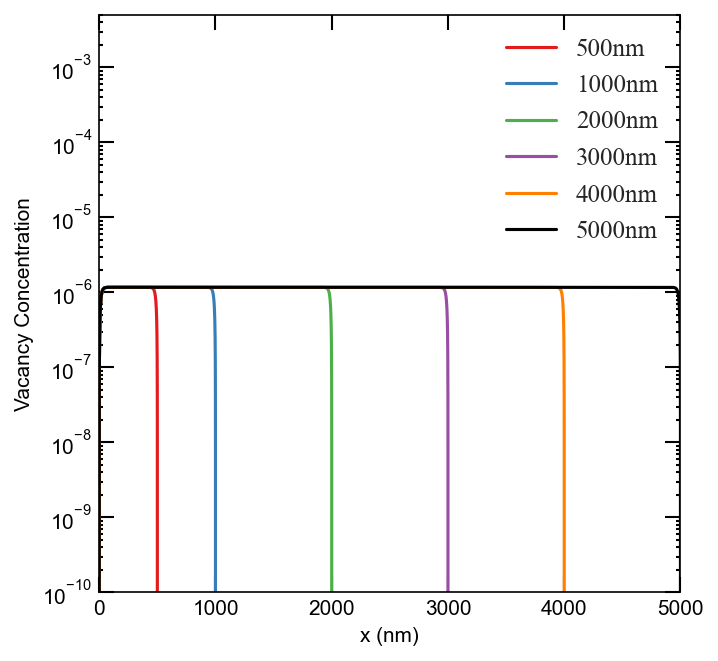
\includegraphics[scale=0.55]{vacancy_concentration_500-5000nm-high_neutron-0}
    %     \caption{Concentration profiles with 0\% production bias, interstitial concentration for a) neutrons and b) protons, vacancy concentration for c) neutrons and b) protons}
    %     \label{figure:concentrations_neutron_0_1e-6}
    % \end{figure}

    Whenever a production bias exists, the steady-state profiles of defects show different trends. Depending on production rate and bias, a critical grain size exists above which the spatial dependence of the interstitial, the defect type with lower production rate, is reversed. This result can be attributed to the fact that production bias breaks the symmetry of the point defect balance leading to the manifestation of distinct steady-state profiles for the different defects. It is worth noting that such instability will make irradiation damage more pronounced.
    Since it will enhance the clustering of different point defects into distinct extended defects, vacancies at the center of the domain will cluster into voids. Simultaneously, interstitials close to the boundaries will form dislocation loops.
    In (\%5) production bias case, we have observed that the steady-state concentration profile has changed significantly. The interstitial concentration at center decreases, and its spatial profile turns down after \textit{critical grain size} (${\sim}$1000 nm in Fig. \ref{figure:concentrations_neutron_5_1e-6}a). Moreover, the depth of profile gets larger with increasing grain size, which could be explained as accumulation of more interstitial atoms trying to reach equilibrium at boundary. On the other hand, the vacancy concentration increases equivalent to grain size, as seen in Fig. \ref{figure:concentrations_neutron_5_1e-6}b.

    Similar to the unbiased case, protons increases average concentration levels. The most significant effect of protons is causing decrease in critical grain size. Therefore, the interstitial concentration profile starts being reversed in smaller grain sizes than 500 nm. (see Fig. \ref{figure:concentrations_proton_5_1e-3}).\\
    \begin{figure}[h!]  %Neutron - 1e-6 dpa/s - %5 Bias rate
        \centering
        a)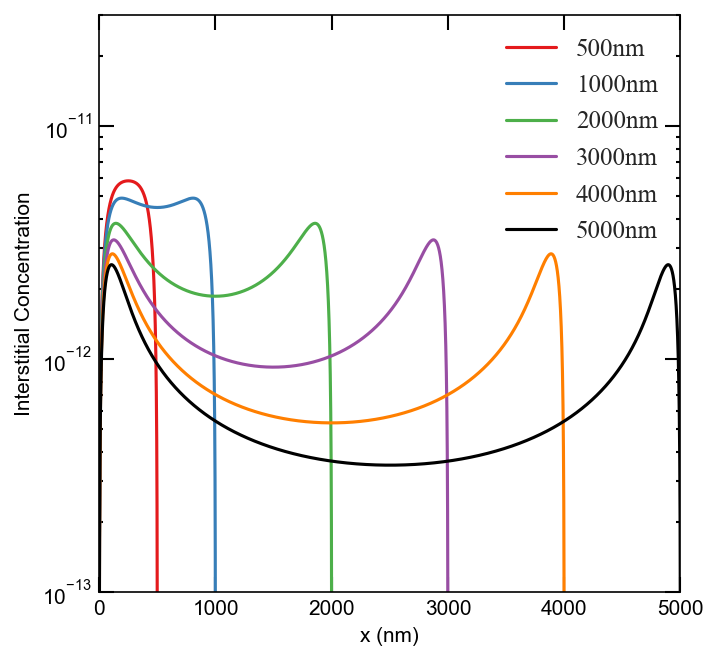
\includegraphics[scale=0.55]{interstitial_concentration_500-5000nm-neutron-5}
        b)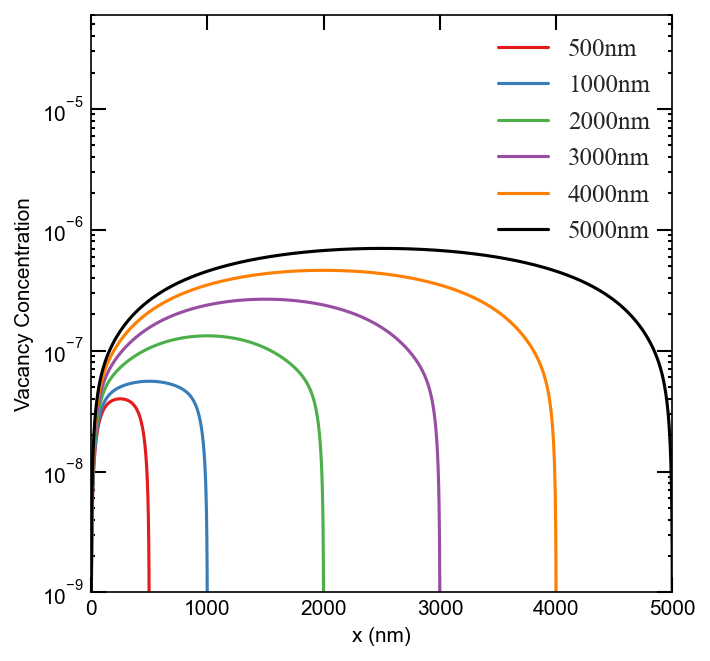
\includegraphics[scale=0.55]{vacancy_concentration_500-5000nm-neutron-5}
        c)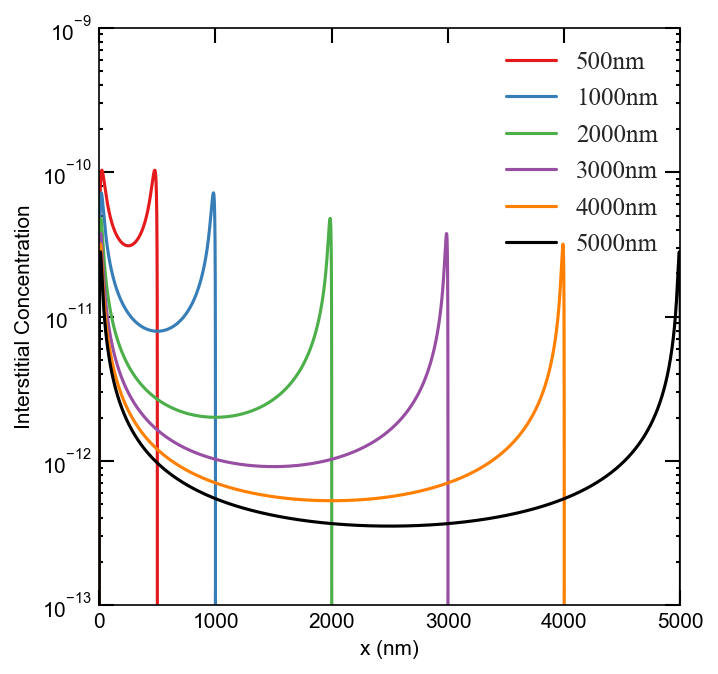
\includegraphics[scale=0.55]{interstitial_concentration_500-5000nm-high_neutron-5}
        d)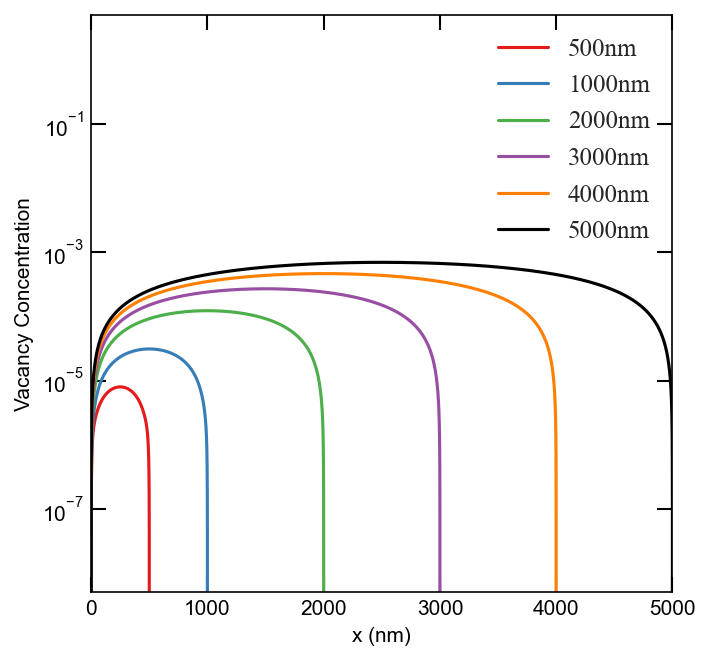
\includegraphics[scale=0.55]{vacancy_concentration_500-5000nm-high_neutron-5}
        e)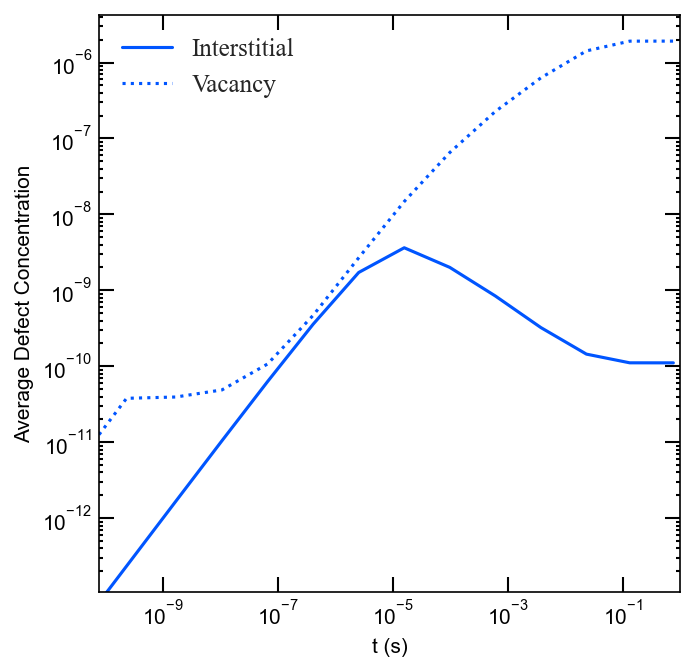
\includegraphics[scale=0.55]{average_concentration_250nm}
        f)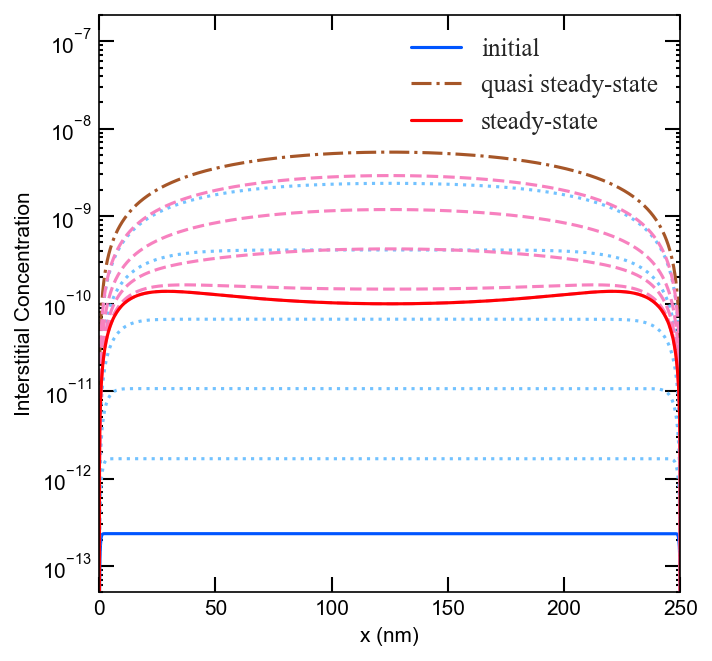
\includegraphics[scale=0.55]{interstitial_concentration_time_evolution_250nm}
        \caption{Concentration profiles with 5\% production bias for neutrons (a,b) and protons (c,d). e) Average defect concentration change with time for ${250nm}$. f) The evolution of interstitial concentration profile for ${250nm}$}
        \label{figure:concentrations_neutron_5_1e-6}
    \end{figure}\\

\textcolor{red}{
change font size //
comment on trends//
1 paragraph//
being radiation tolerant of nanocrystals//
larger grain size increases clustering//
}
\\
\subsubsection{Vacancy Supersaturation}
    Voids are the result of vacancy agglomeration. Therefore,  supersaturated vacancies in microstructure can lead to void formation. Moreover, void formation affects the properties of the material as it will change the material volume. The volume expansion of materials under irradiation is known as void swelling. In order to understand the details of void swelling behavior as a function of irradiation dose rate, the effective vacancy supersaturation is calculated.

    Supersaturation is a condition that the actual concentration of point defect is larger than its equilibrium concentration. The opposite condition is called undersaturation which is being smaller than equilibrium concentration. In both cases, the system is not at the minimum free energy.

    The effective vacancy supersaturation, ${S_v}$ is calculated by using following equation, \citep{was2017}

    \begin{equation}
        \begin{aligned}
        &S_v=\frac{D_vC_v-D_iC_i}{D_vC_v^e}\\
        \end{aligned}
    \end{equation}

    The vacancy supersaturation curves for biased neutron irradiation is given in Fig. \ref{figure:vacancy_supersaturation_neutron}. Since the defect concentrations have symmetrical profiles for neutron irradiation, supersaturation curves are also symmetrical around grain center. The plot shows a non-linear increase in supersaturation values as grain gets larger.

\textcolor{red}{
linear dependence with production rate, non linear dependency with grain size and production bias//
}

    \newpage
    \subsubsection{Grain Boundary Sink Strength}
    The sink reaction term in Eq. \ref{equation:point_defect_equations_sink_strength} represents the total loss of point defects to sinks that are voids and dislocations within the domain. It can be written in expanded form as below,

    \begin{equation}
      \begin{aligned}
        &k^2DC=(Z\rho_d+4\pi r_h\rho_h)DC\\
      \end{aligned}
    \end{equation}\\
    Similarly, grain boundary sink strength can be calculated by considering total flow of point defect to grain boundary.

    \begin{equation}
      \begin{aligned}
        &F=Z_{gb}DC_0\\
        &Z_{gb}=\frac{F}{DC_0}\\
      \end{aligned}
      \end{equation}\\

    where ${F}$ is total flow at grain boundary, ${Z_{gb}}$ is grain boundary sink strength, ${D}$ is diffusion coefficient and ${C_0}$ is defect concentration at the domain center.\\\\
    The total flow at boundary is equal to multiplication of surface area and current as below,\\

    \begin{equation}
      \begin{aligned}
        &F=-\bigg(4\pi r^2D\frac{\partial C(r)}{\partial r}\bigg)_{r=a}\\
      \end{aligned}
    \end{equation}\\
    The total grain boundary sink strength, ${k^2_{gb}}$ is calculated by multiplying ${Z_{gb}}$ by the grain density, ${\rho_{gb}}$. \citep{heald1977}
    \begin{equation}
      \begin{aligned}
        &\rho_{gb}=\frac{6}{\pi d^3}\\
        &k^2_{gb}=\rho_{gb}Z_{gb}\\
      \end{aligned}
    \end{equation}

    where ${d}$ is diameter of the grain, ${d=2a}$\\\\
    Grain boundary sink strengths, ${Z_{gb}}$ and ${k_{gb}}$, is calculated analytically by substituting Eq.  \ref{equation:spherical_grain_analytical_solution} into expressions above. Thus, grain boundary sink strengths are associated with the domain sink strength, ${k^2}$. \citep{heald1977}

    \begin{equation}
      \begin{aligned}
        &C_0=C(r=0)=\frac{K_0}{Dk^2}\bigg(1-\frac{ka}{\sinh{ka}}\bigg)\\\\
        &F=-\bigg(4\pi r^2D\frac{\partial C(r)}{\partial r}\bigg)_{r=a}=\frac{4\pi aK_0}{k^2}\bigg(ka\coth{ka}-1\bigg)\\
      \end{aligned}
    \end{equation}\\
    So that, grain boundary sink strengths are
    \begin{equation}
      \begin{aligned}
        &Z_{gb}=4\pi a\bigg(\frac{ka\cosh ka-\sinh ka}{\sinh ka-ka}\bigg)\\
        &k^2_{gb}=\frac{12}{d^2}\bigg(\frac{ka\cosh ka-\sinh ka}{\sinh ka-ka}\bigg)\\
      \end{aligned}
    \end{equation}\\

    Grain Boundary sink strength for different defect type can be calculated by using appropriate diffusion coefficient (${D}$), domain sink strength (${k^2}$) and concentration (${C_0}$). The analytical expression for each is given by following equations,

    \begin{equation}
      \begin{aligned}
        &Z_{gb,i}=4\pi a\bigg(\frac{k_ia\cosh k_ia-\sinh k_ia}{\sinh k_ia-k_ia}\bigg)\\
        &k^2_{gb,i}=\frac{12}{d^2}\bigg(\frac{k_ia\cosh k_ia-\sinh k_ia}{\sinh k_ia-k_ia}\bigg)\\\\
        &Z_{gb,v}=4\pi a\bigg(\frac{k_va\cosh k_va-\sinh k_va}{\sinh k_va-k_va}\bigg)\\
        &k^2_{gb,v}=\frac{12}{d^2}\bigg(\frac{k_va\cosh k_va-\sinh k_va}{\sinh k_va-k_va}\bigg)\\
      \end{aligned}
    \end{equation}\\

    The results of benchmark problem, previously discussed in Fig. \ref{figure:concentrations_MOOSE_analytical}, can also be used to validate MOOSE sink strength calculations.

    Calculated sink strengths for different grain sizes are shown in Fig \ref{figure:sink_strengths_neutron_5_1e-6}. The grain boundary sink strengths, ${Z^{gb}}$ and ${k^2_i}$, separate from each other after critical grain size value for both neutrons (Fig \ref{figure:sink_strengths_neutron_5_1e-6} a,c) and protons (Fig \ref{figure:sink_strengths_neutron_5_1e-6} b,d). The separation is more significant for protons because of higher dose rate.

    The change of sink strengths with different production bias or grain sizes are presented in 3D surface plot as given in Fig. \ref{figure:sink_strength_moose_neutron_3D}.

\textcolor{red}{
more comment on trends related to grain size, production bias, production rate//
critical grain size $>$ critical size//
}
    \begin{figure}[h!]  %Sink Strength - Neutron 1e-6 dpa/s - 5% Bias rate
        \centering
        a)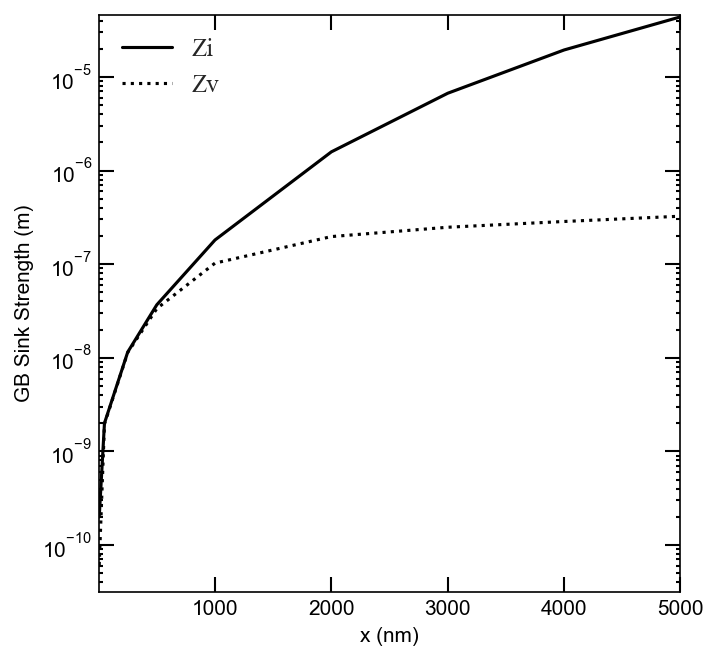
\includegraphics[scale=0.55]{sink_strength_moose_neutron_5_Z_scaled}
        b)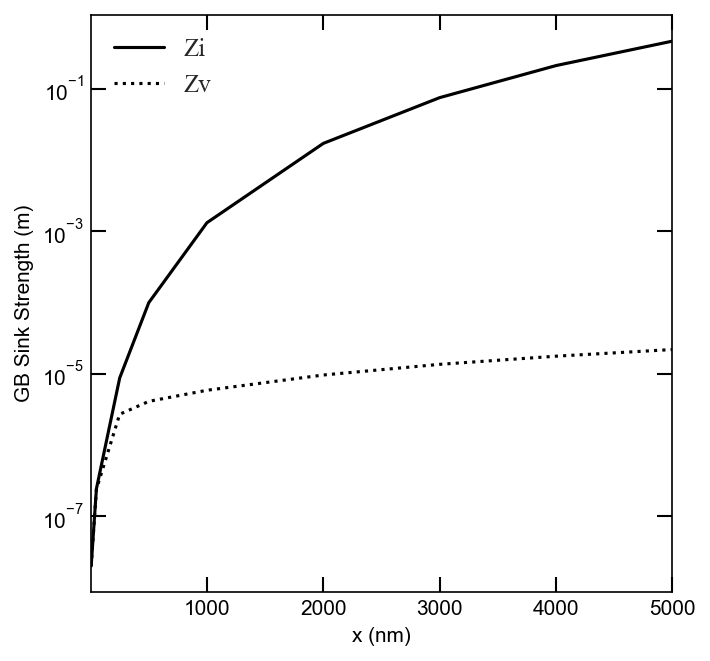
\includegraphics[scale=0.55]{sink_strength_moose_high_neutron_5_Z_scaled}
        \caption{Change of grain boundary sink strengths with grain size for 5\% production bias, a) neutron, b) proton}
        \label{figure:sink_strengths_neutron_5_1e-6}
    \end{figure}

    \begin{figure}[h!]  %GB Sink Strength - Neutron 1e-6 dpa/s
        \centering
        a)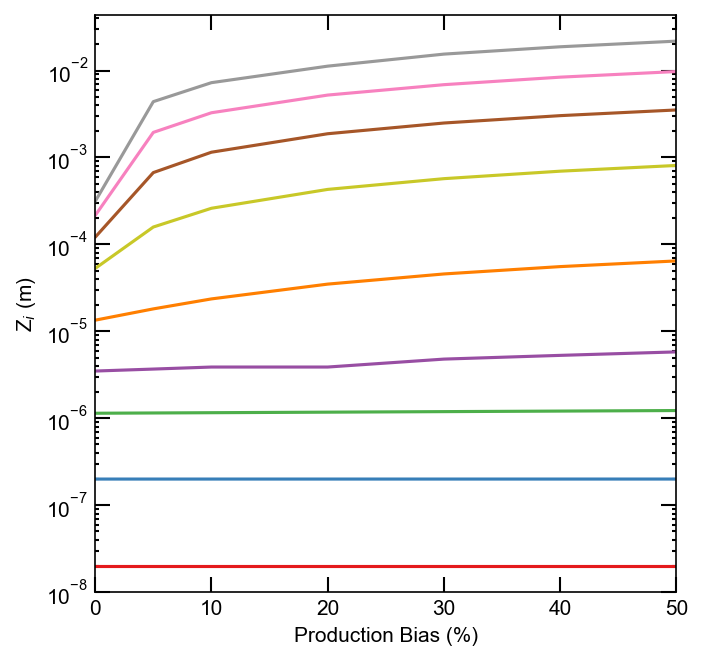
\includegraphics[scale=0.55]{sink_strength_neutron_Zi_scaled_nolegend}
        b)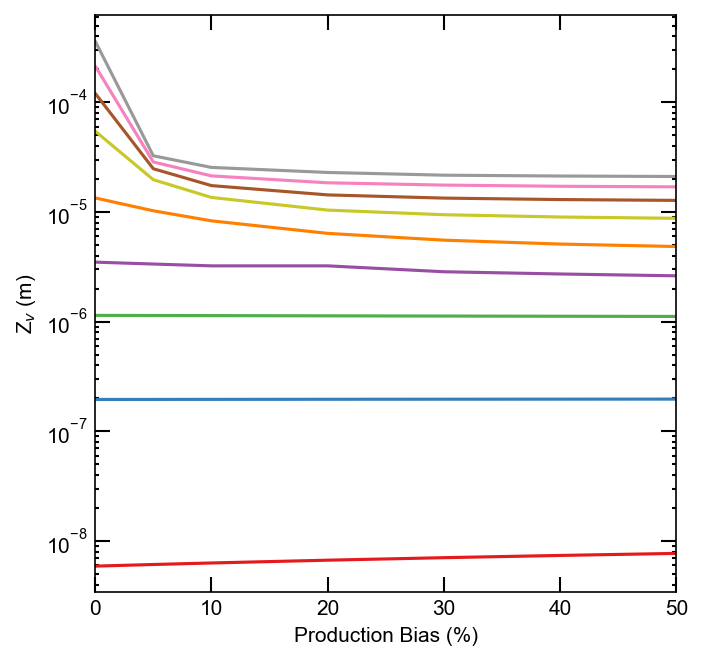
\includegraphics[scale=0.55]{sink_strength_neutron_Zv_scaled_nolegend}
        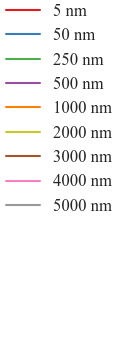
\includegraphics[scale=0.35]{legend}
        c)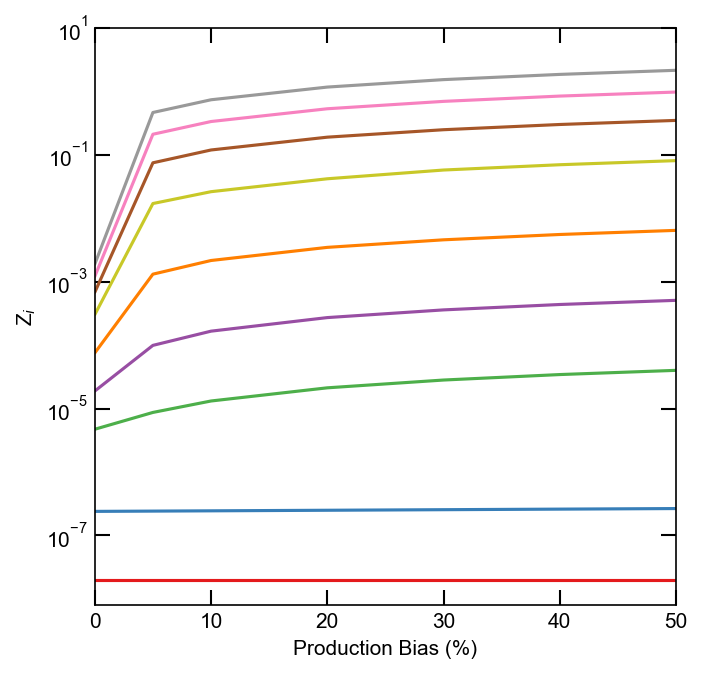
\includegraphics[scale=0.55]{sink_strength_high_neutron_Zi_scaled_nolegend}
        d)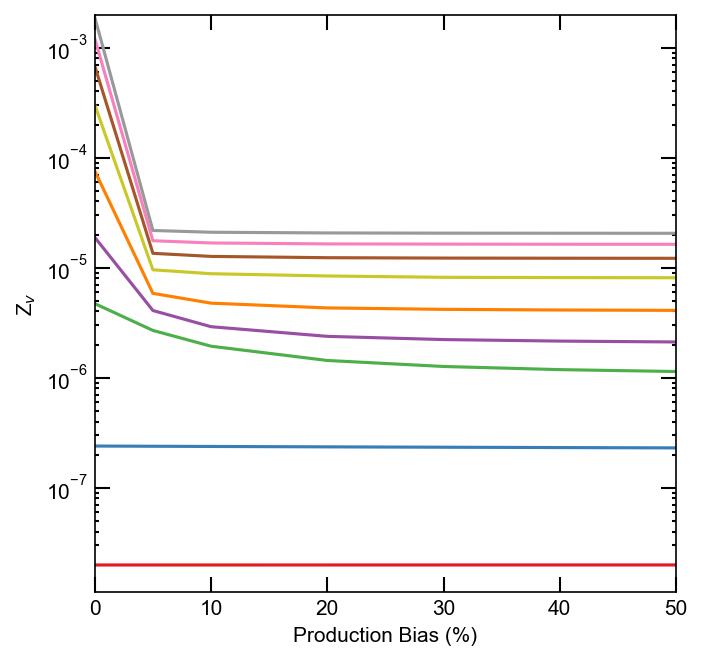
\includegraphics[scale=0.55]{sink_strength_high_neutron_Zv_scaled_nolegend}
        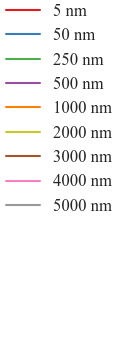
\includegraphics[scale=0.35]{legend}
        \caption{Change of grain boundary sink strengths with production bias and grain size for neutrons (a,b) and protons (c,d)}
        \label{figure:sink_strengths_neutron_bias_Z}
    \end{figure}

    %   \begin{figure}[h!]  %Sink Strength 3D - Neutron 1e-6 dpa/s
    %     \centering
    %     a)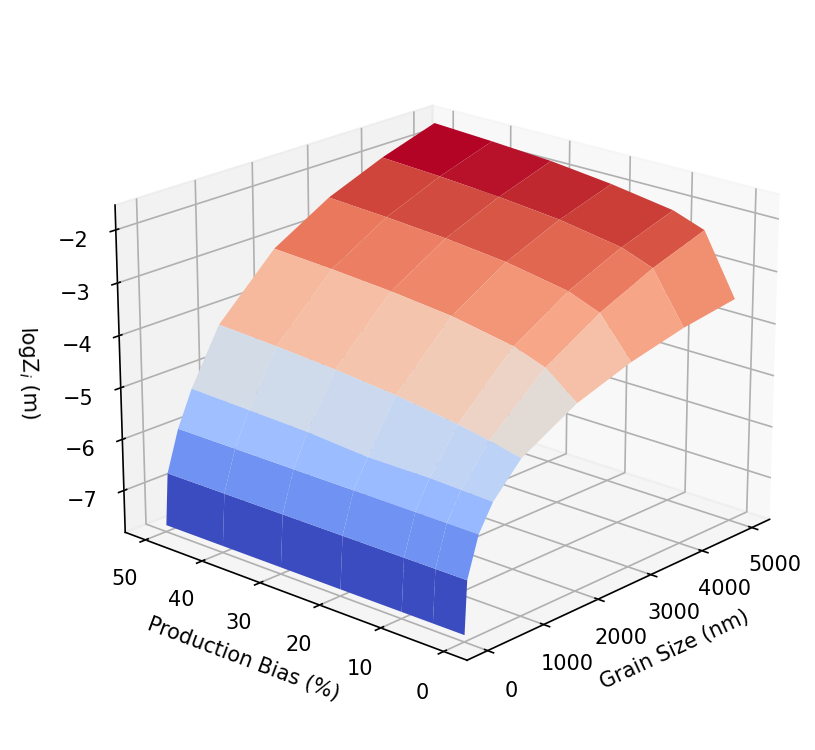
\includegraphics[scale=0.55]{sink_strength_moose_neutron_3D_Zi_scaled}
    %     b)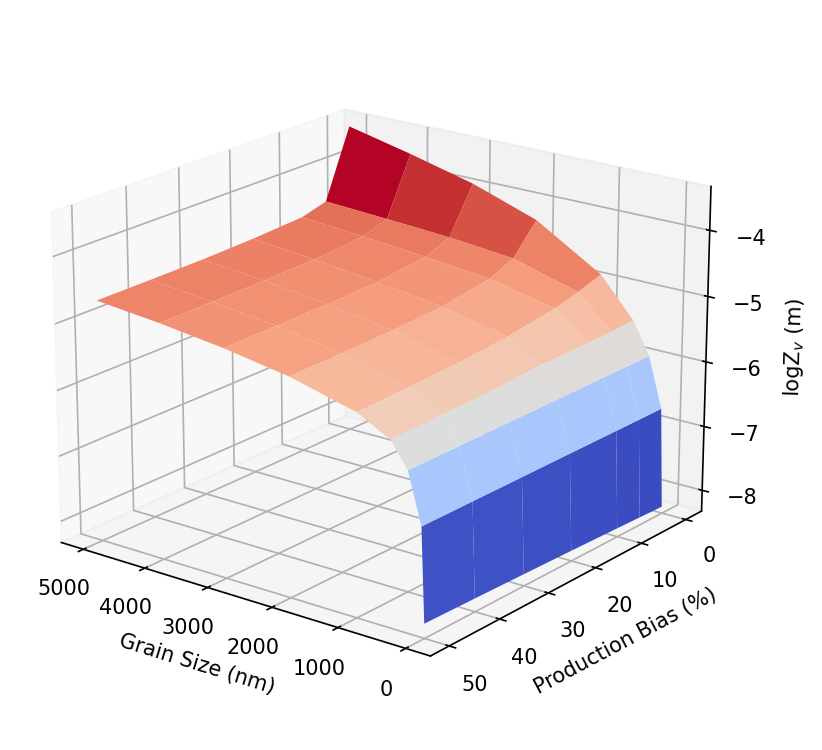
\includegraphics[scale=0.5]{sink_strength_moose_neutron_3D_Zv_scaled}
    %     c)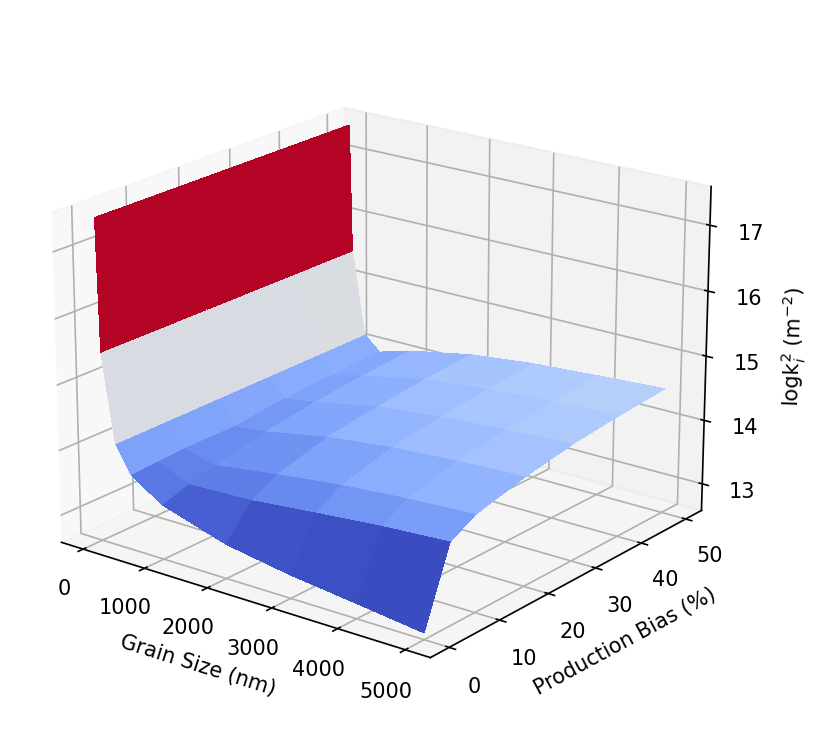
\includegraphics[scale=0.55]{sink_strength_moose_neutron_3D_ki_scaled}
    %     d)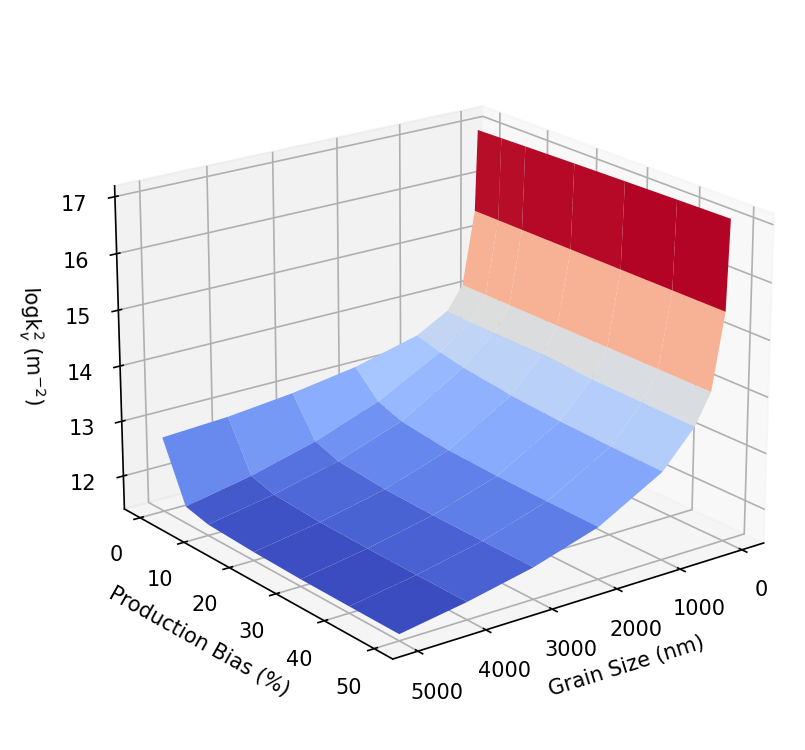
\includegraphics[scale=0.55]{sink_strength_moose_neutron_3D_kv_scaled}
    %     \caption{Change of sink strengths with grain size and production bias for neutrons in log scale, a)interstitial grain boundary sink strength, b) vacancy grain boundary sink strength, c) total interstitial grain boundary sink strength, d) total vacancy grain boundary sink strength}
    %     \label{figure:sink_strength_moose_neutron_3D}
    %   \end{figure}

\clearpage
\subsection{Non-Uniform Irradiation}
    Contrary to neutrons, ions have a relatively narrow energy channel width, which is almost monoenergetic. Furthermore, they cannot penetrate through material excessively because of their high energy loss in collisions. This characteristic behavior causes a non-uniform defect production profile. Figure \ref{figure:defect_production} shows the profile used for ion irradiation simulations. The dose rate, K\textsubscript{0} and grain size (1000 nm) would be scaled for the case of interest, but it does not create a change in the profile.
    \begin{figure}[h!]  %Ion irradiation
        \centering
        a)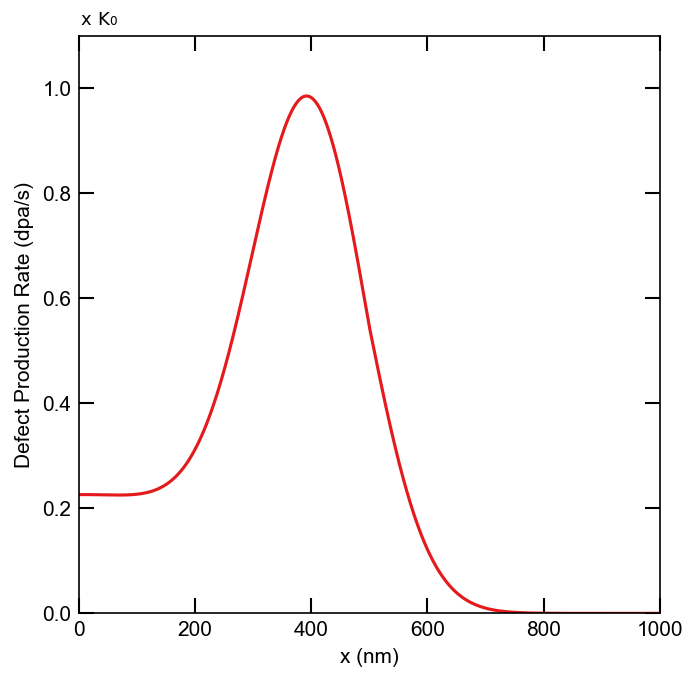
\includegraphics[scale=0.27]{defect_production}
        \qquad
        b)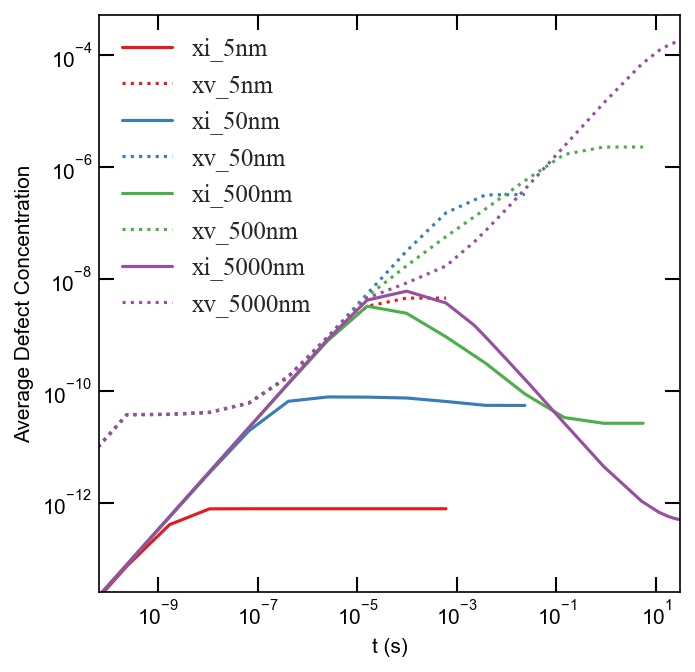
\includegraphics[scale=0.55]{average_concentration_ion_5_size}
        \caption{a)Defect production profile for ion irradiation, b)Time-dependent behavior of average defect concentration  with 5\% production bias for ions}
        \label{figure:defect_production}
    \end{figure}
\subsubsection{Concentrations}
    Even though ion irradiation has non-uniform defect production, average defect concentrations show a time-dependent trend that is identical to the one in neutron irradiation case. The only difference is the change in concentration levels as a result of less defect production (see Fig. \ref{figure:average_concentrations_ion_5}).

    The effect of defect production distribution can be observed obviously in concentration profiles. Since, defect production has peak at around half of the grain, the concentration profiles are taking shape under same behavior and reaching maximum at the center of domain, then waning through boundaries.

    If production bias is zero, maximum concentration of each type of point defect becomes independent of grain sizes shown in Fig. \ref{figure:concentrations_ion_0_1e-3}).

    %   \begin{figure}[h!]  %Ion - 1e-3 dpa/s - %0 Bias rate
    %     \centering
    %     a)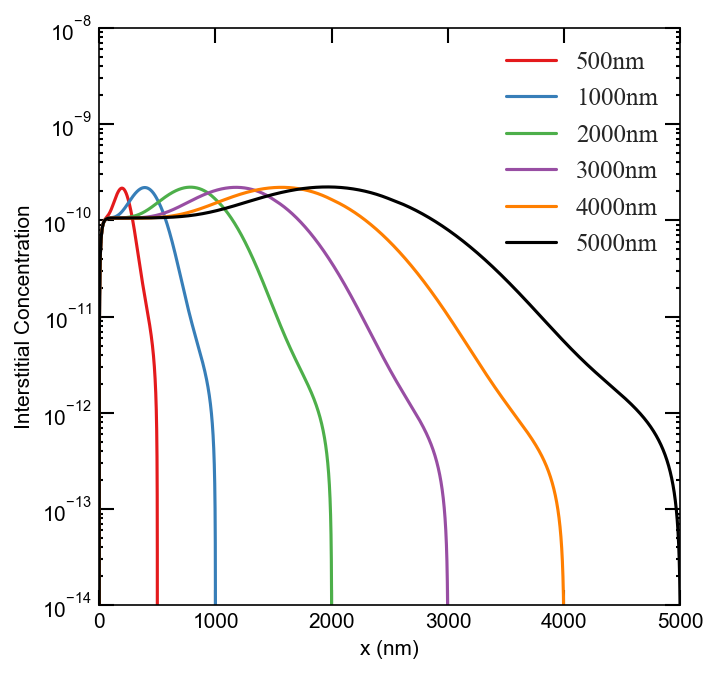
\includegraphics[scale=0.55]{interstitial_concentration_500-5000nm-ion-0}
    %     b)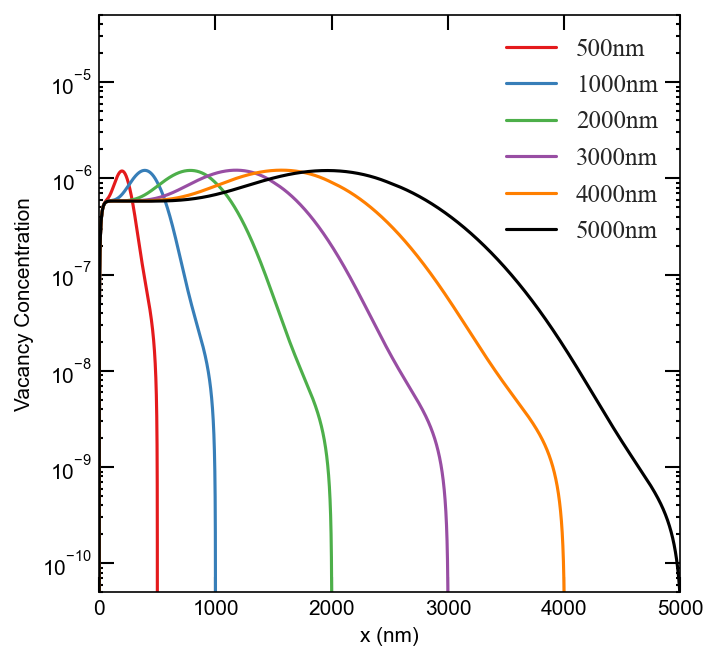
\includegraphics[scale=0.55]{vacancy_concentration_500-5000nm-ion-0}
    %     \caption{Concentration profiles for ions with 0\% production bias, a) interstitial concentration, b) vacancy concentration}
    %     \label{figure:concentrations_ion_0_1e-3}
    %   \end{figure}

    In the case of applying production bias, profiles become completely different. In addition to the reversal behavior observed in neutron irradiation case, the non-uniform defect production profile causes asymmetrical interstitial concentration profile as given in Fig. \ref{figure:concentrations_ion_5_1e-3}a. The critical grain size for ion case occurs around ${\sim}$1000 nm. The vacancy concentration profiles also loose their symmetry and shift up with increasing grain size (see Fig. \ref{figure:concentrations_ion_5_1e-3}b).

      \begin{figure}[h!]  %Ion - 1e-3 dpa/s - %5 Bias rate
        \centering
        a)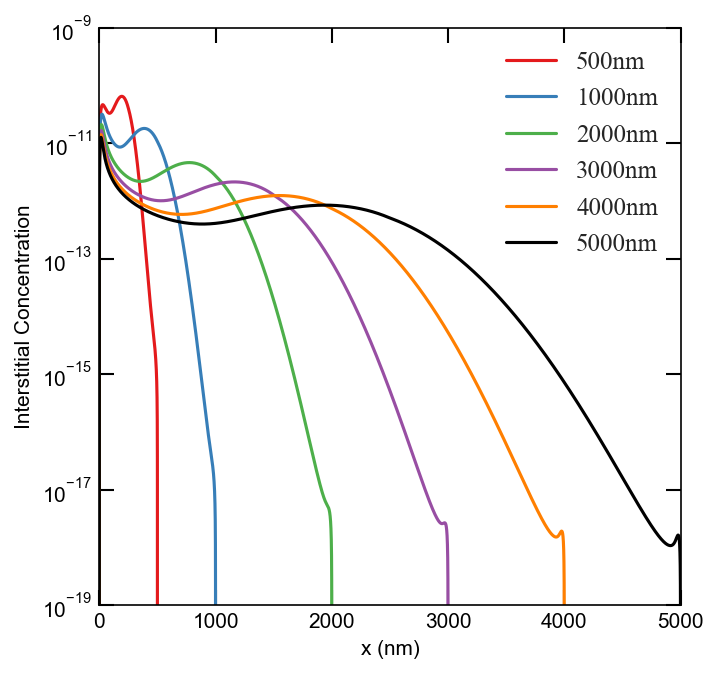
\includegraphics[scale=0.55]{interstitial_concentration_500-5000nm-ion-5}
        b)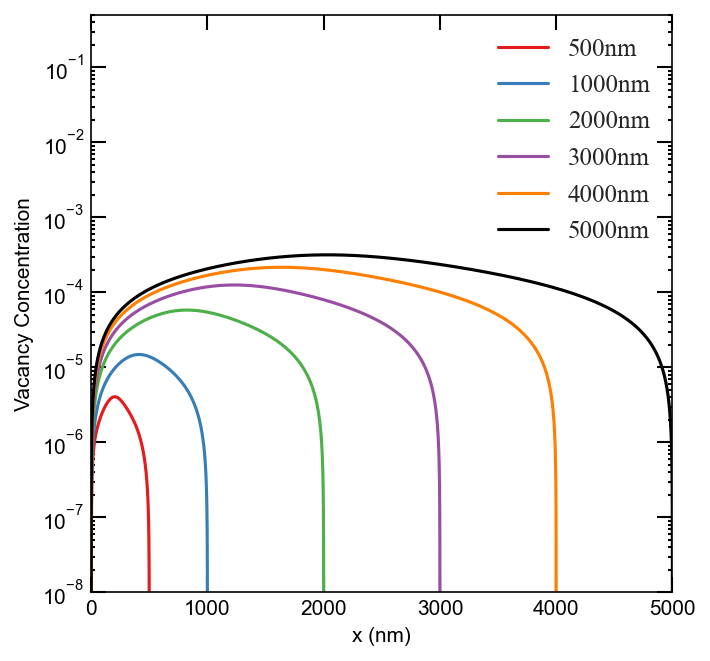
\includegraphics[scale=0.55]{vacancy_concentration_500-5000nm-ion-5}
        \caption{Concentration profiles for ions with 5\% production bias, a) interstitial concentration, b) vacancy concentration}
        \label{figure:concentrations_ion_5_1e-3}
      \end{figure}

\newpage
\subsubsection{Vacancy Supersaturation}
    The vacancy supersaturation curves for ion irradiation case are quite similar to ones for neutron irradiation case. The only difference is the asymmetrical shape of curves originates from concentration profiles. The non-linear increase in supersaturation values as domain gets larger is observed for ion irradiation too.
    %\textcolor{blue}
    The vacancy supersaturation behavior, shown in Fig. \ref{figure:vacancy_supersaturation_ion}, is identical to one in given for neutron irradiation case (see Fig. \ref{figure:vacancy_supersaturation_neutron}). The only difference is the asymmetrical shape of curves originating from defect production distribution. This similarity makes it possible to use ions instead of neutrons to predict the swelling behavior of reactor materials. The non-linear increase in supersaturation peak values might result in more void creation and undesired swelling behavior.\\

\subsubsection{Grain Boundary Sink Strength}
    The sink strengths are directly related to concentration at center and flow at boundary. The change of defect concentrations are not as considerable as neutron case. So, the flow or flux at boundary becomes more dominant on sink strength profiles (see Fig. \ref{figure:sink_strengths_ion_5_1e-3}c).

    As discussed previously, since ions can not penetrate until the end of the domain, they cause a non-uniform defect production. If the grain is small enough compared to penetration depth, concentration profiles become symmetrical (similar to neutron case), and the effect of distribution profile is not visible (up to 1000 $nm$ in Fig. \ref{figure:concentrations_ion_5_1e-3_5-5000nm}). Yet, for larger grains, the defect concentrations are highly affected by non-uniformity. The flux at the far boundary oscillates and approaches zero as grain size increases. Since sink strengths are related to the ratio of flux to concentration, they are affected by those oscillations.

    \begin{figure}[h!]  %Sink Strength - ion 1e-3 dpa/s - 5% Bias rate
        \centering
        a)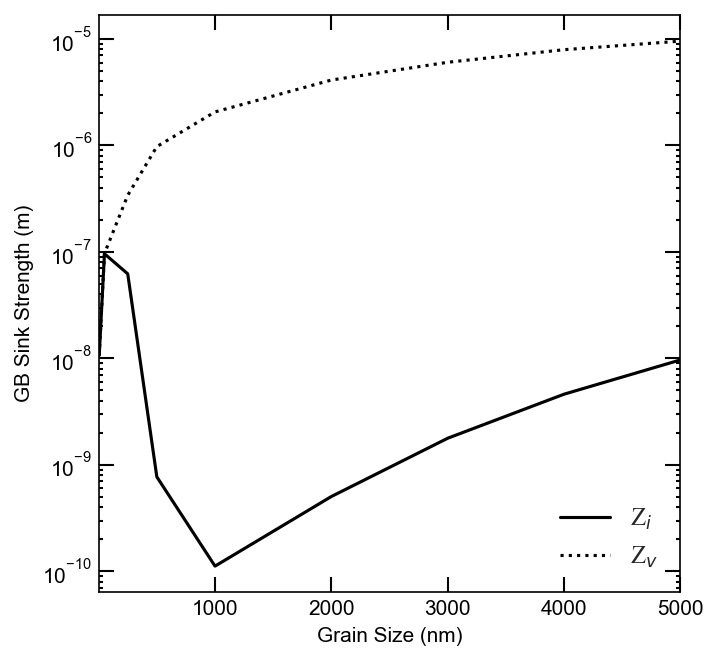
\includegraphics[scale=0.55]{sink_strength_moose_ion_5_Z_scaled}
        b)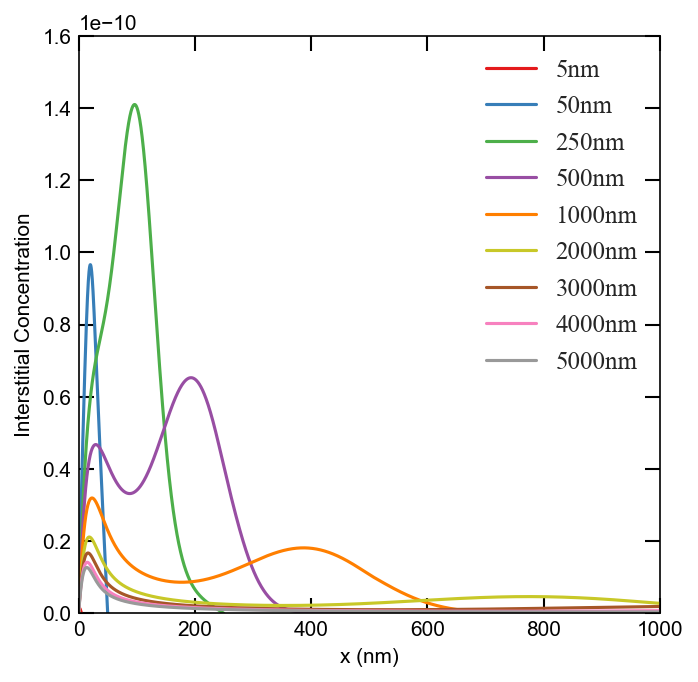
\includegraphics[scale=0.55]{interstitial_concentration_5-5000nm-ion-5}
        \caption{a) Change of grain boundary sink strengths with grain size for 5\% production bias for ions, b) Change of interstitial concentration for different grain sizes}
        \label{figure:sink_strengths_ion_5_1e-3}
    \end{figure}

    \begin{figure}[h!]  %GB Sink Strength - Ion 1e-3 dpa/s
        \centering
        a)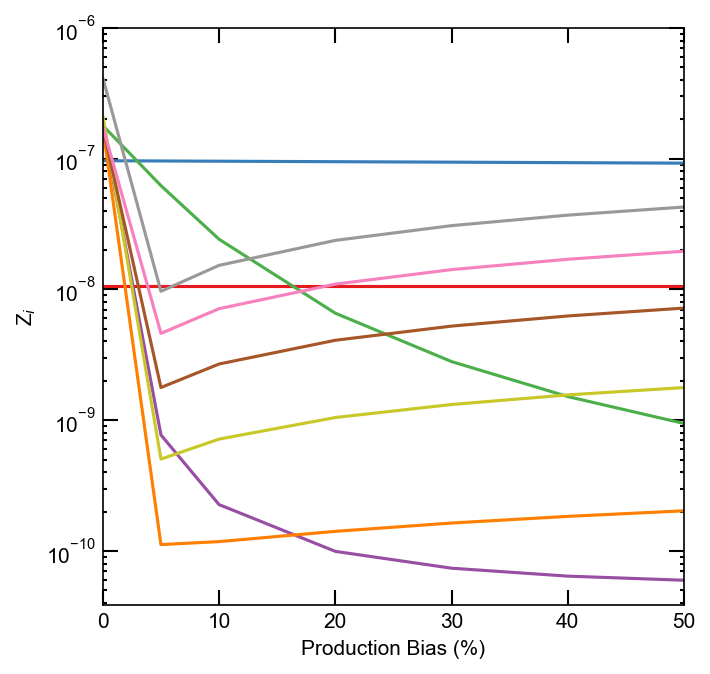
\includegraphics[scale=0.55]{sink_strength_ion_Zi_scaled_nolegend}
        b)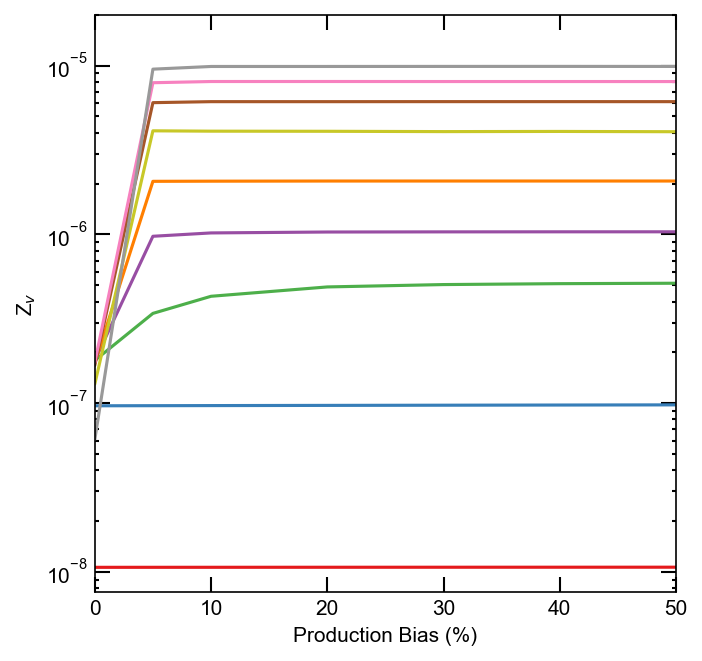
\includegraphics[scale=0.55]{sink_strength_ion_Zv_scaled_nolegend}
        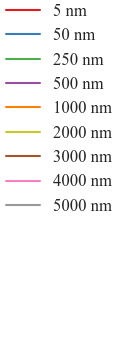
\includegraphics[scale=0.35]{legend}
        \caption{Change of grain boundary sink strengths with production bias and grain size for ions}
        \label{figure:sink_strengths_ion_bias_Z}
    \end{figure}
\newpage
\subsection{Radiation-induced Segregation}

    Ni-Cr based alloys is one of the most important structural materials for current and future advanced fission reactor designs. Currently, Ni-Cr based alloys are used widely in light water reactors (LWR), particularly for reactor coolant systems. These alloys show high strength and resistance to swelling at high temperatures and superior corrosion performance. Despite their many advantages, however, irradiation may cause dramatic changes to composition of alloy following that radiation induced segregation (RIS) can take place near microstructural defects where materials are sensitive to corrosive attack. Point defects can migrate, recombine, and cancel each other out on numerous sinks i.e., dislocations, free surfaces, or grain boundaries. The migration of these point defects causes significant changes in microstructure with similar changes in behavior. Ni-Cr based alloys contains a high Cr content to prevent corrosion. The decrease in the local composition of Cr may result in severe structural changes. Predictions of the effects of RIS in Ni-Cr based alloys are crucial for determining safe limits in the work environment.

    In this section, in order to understand the effect of production bias on the various spatial profile of atom and defect concentrations, we used 5\%, 10\%, and 20\% production bias factors to produce a difference between interstitial and vacancy generation.
    \\
    \subsubsection{Rate Theory model for RIS}

    This model considers the coupling of defects and atom fluxes through migration of interstitials and vacancies in a binary Ni-Cr alloy.

    \begin{equation}
        \begin{aligned}
        &\frac{dC_i}{dt} = - \nabla\cdot J_i + K_0 - K_{iv}C_iC_v - S \\
        &\frac{dC_v}{dt} = - \nabla\cdot J_v + K_0 - K_{iv}C_iC_v - S\\
        &\frac{dC_{Cr}}{dt} = - \nabla\cdot J_{Cr} \\
        \end{aligned}
        \label{equation:RIS_equations}
     \end{equation}\\
    In the above, $\nabla\cdot J_i$ and $\nabla\cdot J_v$ are the divergences of the vacancy and interstitial fluxes at defect sinks, and $K_0$, $K_{iv}C_IC_V$, S terms are the local total rates of production, recombination of point defects per unit volume and sink absorption rate respectively.
    Vacancy and interstitial concentrations were determined as the concentrations at thermal equilibrium for the initial conditions of system. Cr concentration is taken as the nominal value in the alloy composition. We assume that the alloy atoms are randomly distributed throughout the grain at the initial time. The equations were solved numerically with the initial and boundary conditions, and one-dimension calculations were performed.

    \begin{table}[h!]
  \centering
  \caption{Input Parameters for RIS }
  \label{table:Input_parameters_for_RIS}
  \begin{tabular}{ ||p{7cm}|p{1cm}|p{2cm}||p{1cm}|p{1.5cm}||  }
     % \hline
     % \multicolumn{5}{|c|}{Material Properties} \\
     \hline
     Input Parameter & Symbol & Value & Units &  Reference\\
     \hline\hline

     Vacancy jump frequency for Ni & \omega_{Ni,v}  & 0 & s^{-1} &\\
     Vacancy jump frequency for Cr & \omega_{Cr,v}  & 0 & s^{-1} &\\
     Interstitial jump frequency for Ni & \omega_{Ni,,i}  & 0 & s^{-1} &\\
     Interstitial jump frequency for Cr & \omega_{Cr,i}  & 0 & s^{-1} &\\
     Vacancy migration energy for Ni & E_{Ni,v}^m  & 0 & eV & \\
     Vacancy migration energy for Cr & E_{Cr,v}^m  & 0 & eV & \\
     Interstitial migration energy for Ni & E_{Ni,i}^m  & 0 & eV & \\
     Interstitial migration energy for Cr  & E_{Cr,i}^m  & 0 & eV & \\
     Vacancy jump correlation factor for Ni  & f_vNi  & 0 & unitless & \\
     Vacancy jump correlation factor for Cr  & f_vCr  & 0 & unitless & \\
     Interstitial jump correlation factor for Ni   & f_iNi  & 0 & unitless & \\
     Interstitial jump correlation factor for Cr  & f_iCr  & 0 & unitless & \\
     \hline
  \end{tabular}
\end{table}

    \begin{equation}
        \begin{aligned}
        d_{z}^{v,i}\ =\frac{1}{6}\lambda^2 \omega f exp(\frac{-E_{z-v,i}^m}{k_B T})
        \end{aligned}
        \label{equation:RIS_equations}
    \end{equation}\\
    $d_{a}^{v,i}$ represents diffusivity coefficient for the atom-defect pairs. For the chosen z atom, in this work z is Ni and Cr atoms, $\lambda$ is jump distance, $\omega$ is jump frequency and f is correlation factor. For vacancy and interstitial, $E_{z-v,i}^m$ is migration energy and $k_B$ is Boltzmann constant.


    RIS behavior in the alloy with Ni-18Cr composition shows a vacancy-driven inverse Kirkendall mechanism. While chromium diffuses rapidly with vacancy flux, the concentration of chromium decreases at the grain boundaries, and the concentration of Nickel moving slower than Chromium increases at the grain boundary.

    The concentration profiles of defects and Cr atoms at various production biases and grain sizes are presented in Figure \ref{figure:RIS}. Results show that at 50 nm grain size, effect of 5\%, 10\%, and 20\% production bias on interstitials does not show reversal behavior. Yet, at the grain size of 500 nm, the production bias effect shows reversal behavior on interstitials concentration. This conclusion also influences the Cr concentration profile.\\
    The most critical consequence of the reversal behavior and sink density is that fast interstitials find sinks before vacancies. As a result of the interstitials finding sinks faster than vacancies, vacancy concentration continues to increase. This competition between interstitial and vacancy results in interstitials disappearing at the sink and recombining with vacancies.


      \begin{figure}[h!]  %
        \centering
        a)\includegraphics[scale=0.55]{RIS_50nm_vacancy_concentraiton_bias.png}
        b)\includegraphics[scale=0.55]{RIS_500nm_vacancy_concentration_bias.png}
        \\
        c)\includegraphics[scale=0.55]{RIS_50nm_interstitial_concentration_bias.png}
        d)\includegraphics[scale=0.55]{RIS_500nm_interstitial_concentration_bias.png}
        \\
        e)\includegraphics[scale=0.55]{RIS_50nm_chromium_concentration_bias.png}
        f)\includegraphics[scale=0.55]{RIS_500nm_chromium_concentration_bias.png}
        \caption{Concentration profiles for high dose rate neutron with 0\%, 5\%, 10\%, and 20\% production bias a) 50 nm, vacancy concentration b) 500 nm, vacancy concentration c) 50 nm, interstitial concentration d) 500 nm, interstitial concentration e) 50 nm, chromium concentration f) 500 nm, chromium concentration }
        \label{figure:RIS}
      \end{figure}

\clearpage

    Fig.\ref{figure:RIS_Cr_concentration} shows the Cr concentration varying according to grain sizes and production bias. In Fig.\ref{figure:RIS_Cr_concentration}a, the vacancies and interstitials have the same generation rate. The change in Cr concentration profile between 50 and 1000 grain sizes is insignificant. We can say that as the grain size increases, the Cr segregation profile change is observed, but it is not marked clearly. With the purpose of effect of production bias, the production generation was re-analyzed with 20\% bias in the calculations. Fig.\ref{figure:RIS_Cr_concentration}b displays the Cr segregation profiles calculated with 20\% production bias in various grain sizes.  It has been recognized that the area of Cr segregation increases with the increase of production bias and grain size.

    \begin{figure}[h!]  %
        \centering
        a)\includegraphics[scale=0.55]{RIS_domainsize_all.png}
        b)\includegraphics[scale=0.55]{RIS_domainsize_all_20.png}
        \caption{Chromium concentration profiles with a) 0\% and b) 20\% production bias }
        \label{figure:RIS_Cr_concentration}
    \end{figure}


        Trends in radiation-induced segregation in Ni-18Cr alloy occur with Cr depletion. The significance of the Cr segregation, related to the combination of production bias and domain size.\\

        To examine the segregation effect at low temperature and high temperature, low-temperature 200\degree C, high-temperature 800\degree C, and 500\degree C temperature were selected as parameters. For Ni-18Cr alloy, Cr depletion was seen in the range from 200\degree C to 800\degree C. However, the highest Cr depletion effect was 20\% bias at 500\degree C. In general, it was observed that Cr depletion at 200\degree C increased at 500\degree C and decreased again at 800\degree C. It was found that this effect continues to increase in direct proportion to the increase in the production bias effect.\\

        20\% production bias at 500\degree C shows the most remarkable Cr depletion effect, followed by 10\%  production bias at the same temperature. At high temperatures, the amount of Cr depletion is effectively reduced in the grain boundary. This may be due to the fact that at high temperatures, the interstitial concentration began to dominate the vacancy concentration.

    \begin{figure}[h!]  %
        \centering
        a)\includegraphics[scale=0.55]{RIS_1vs10vs20_473_773_1073_Cr_conc.png}
        b)\includegraphics[scale=0.55]{RIS_1vs10vs20_473_773_1073_interstitial_conc.png}
        c)\includegraphics[scale=0.55]{RIS_1vs10vs20_473_773_1073_vacancy_conc.png}
        \caption{Concentration profiles at different temperatures and with 1\%, 10\% and 20\% bias a) chromium b) vacancy and c) interstitial concentration}
        \label{figure:RIS_temperature}
    \end{figure}



\clearpage

  \subsection{Discussion} \hspace{10pt}

    \begin{figure}[htb!]  %Neutron - 1e-6 dpa/s - %5 Bias rate
        \centering
        a)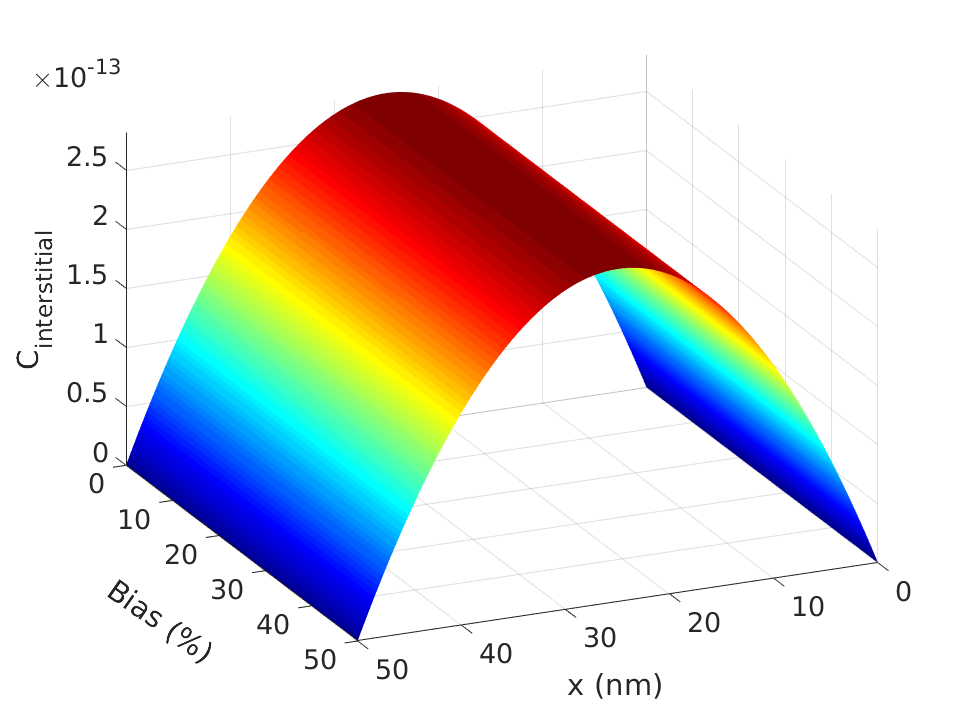
\includegraphics[scale=0.33]{data_neutron_50nm}
        b)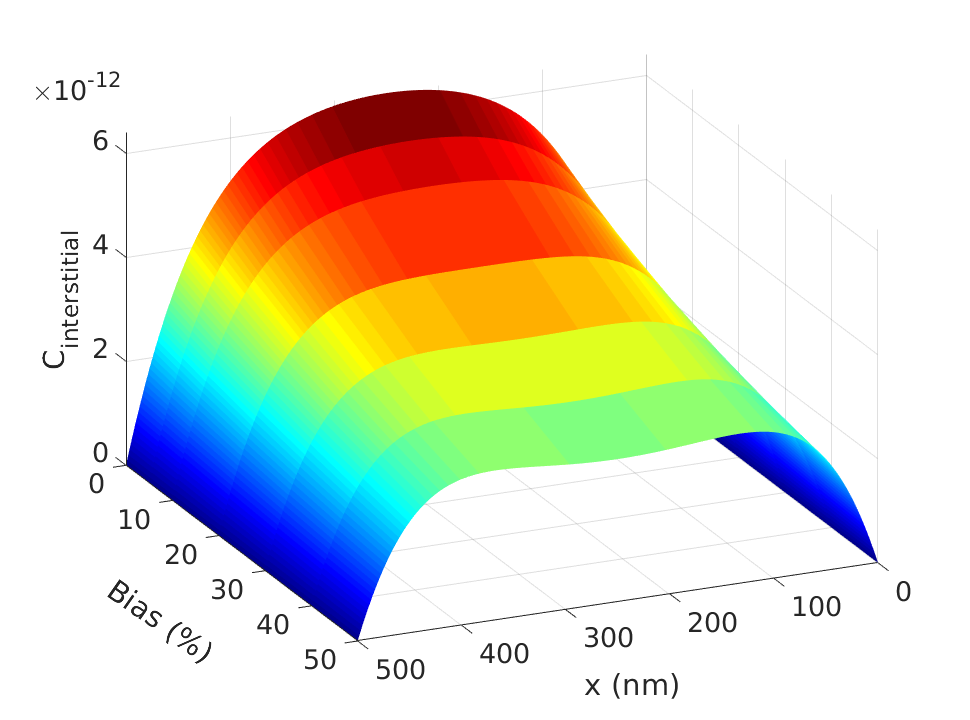
\includegraphics[scale=0.33]{data_neutron_500nm}
        c)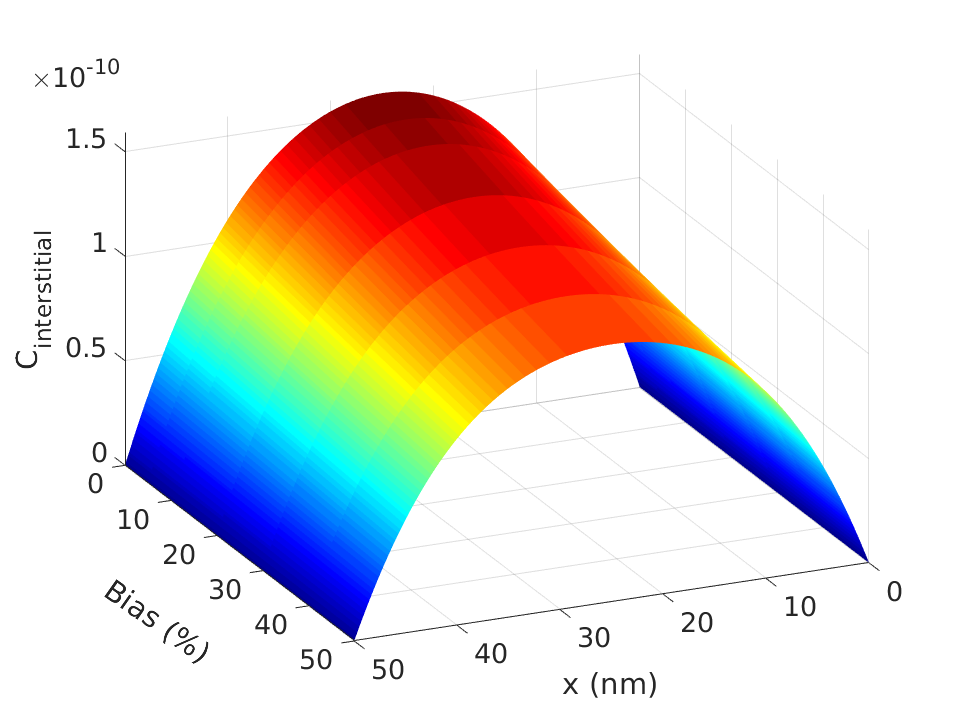
\includegraphics[scale=0.33]{data_high_neutron_50nm}
        d)\includegraphics[scale=0.33]{data_high_neutron_500nm}
        e)\includegraphics[scale=0.33]{data_ion_50nm}
        f)\includegraphics[scale=0.33]{data_ion_500nm}
        f)\includegraphics[scale=0.3]{data_ion_1000nm_grey}
        f)\includegraphics[scale=0.33]{data_ion_1000nm}
        \caption{Change of interstitial concentration profiles with production bias in a grain of 50 $nm$ and 500 $nm$ for neutrons (a,b), protons (c,d) and ions (e,f)}
        \label{figure:3D_concentrations_neutron_1e-6}
    \end{figure}

        \begin{figure}[h!]  %Neutron - Vacancy Supersaturation - 5% Bias
        \centering
        a)\includegraphics[scale=0.55]{super_saturation_500-5000nm-neutron-5}
        b)\includegraphics[scale=0.38]{data_neutron_Sv_center}
        c)\includegraphics[scale=0.55]{super_saturation_500-5000nm-high_neutron-5}
        d)\includegraphics[scale=0.38]{data_high_neutron_Sv_center}
        e)\includegraphics[scale=0.55]{super_saturation_500-5000nm-ion-5}
        f)\includegraphics[scale=0.38]{data_ion_Sv_center}
        \caption{Vacancy supersaturation profiles with different production biases for neutrons and b) protons c) ions, different production biases for neutrons (a,b), protons (c,d) and ions (e,f).  2D plots (a,c,e) shows change of profiles for 5\% production bias.}
        \label{figure:vacancy_supersaturation_neutron}
    \end{figure}

  What happens when switched from neutron irradiation to ion irradiation
  \begin{enumerate}
    \item Loosing symmetry/uniformity in concentration profiles
    \item Reduction in average concentration
    \item Reduction in supersaturation
  \end{enumerate}

\clearpage
\section{Conclusion} \hspace{10pt}

The rate theory equations resolve the temporal and spatial concentration profiles of point defects. The behavior of concentration distributions are controlled by parameters given in equation, representing their reactions and diffusion in domain. According to the results obtained in this study, the combination of production bias, production dose rate, production profile and grain size determine whether the steady state point defect concentration profile is symmetrical, reversed or both. There is always a critical value for parameters that could change the defect concentration profile entirely.
The dependence of radiation induced segregation (RIS) on production biases and grain sizes was reproduced. Results shows that a combination of production bias and grain size results in the change of Cr segregation area.


\clearpage
\bibliographystyle{frontiersinSCNS_ENG_HUMS} % for Science, Engineering and Humanities and Social Sciences articles, for Humanities and Social Sciences articles please include page numbers in the in-text citations
%\bibliographystyle{frontiersinHLTH&FPHY} % for Health, Physics and Mathematics articles
\bibliography{references}

%%% Make sure to upload the bib file along with the tex file and PDF
%%% Please see the test.bib file for some examples of references

\end{document}

% \section{Manuscript Formatting}

% \subsection{Heading Levels}

% %There are 5 heading levels

% \subsection{Level 2}
% \subsubsection{Level 3}
% \paragraph{Level 4}
% \subparagraph{Level 5}

% \subsection{Equations}
% Equations should be inserted in editable format from the equation editor.

% \begin{equation}
% \sum x+ y =Z\label{eq:01}
% \end{equation}

% \subsection{Figures}
% Frontiers requires figures to be submitted individually, in the same order as they are referred to in the manuscript. Figures will then be automatically embedded at the bottom of the submitted manuscript. Kindly ensure that each table and figure is mentioned in the text and in numerical order. Figures must be of sufficient resolution for publication \href{http://home.frontiersin.org/about/author-guidelines#ResolutionRequirements}{see here for examples and minimum requirements}. Figures which are not according to the guidelines will cause substantial delay during the production process. Please see \href{http://home.frontiersin.org/about/author-guidelines#GeneralStyleGuidelinesforFigures}{here} for full figure guidelines. Cite figures with subfigures as figure \ref{fig:2}B.


% \subsubsection{Permission to Reuse and Copyright}
% Figures, tables, and images will be published under a Creative Commons CC-BY licence and permission must be obtained for use of copyrighted material from other sources (including re-published/adapted/modified/partial figures and images from the internet). It is the responsibility of the authors to acquire the licenses, to follow any citation instructions requested by third-party rights holders, and cover any supplementary charges.
% %%Figures, tables, and images will be published under a Creative Commons CC-BY licence and permission must be obtained for use of copyrighted material from other sources (including re-published/adapted/modified/partial figures and images from the internet). It is the responsibility of the authors to acquire the licenses, to follow any citation instructions requested by third-party rights holders, and cover any supplementary charges.

% \subsection{Tables}
% Tables should be inserted at the end of the manuscript. Please build your table directly in LaTeX.Tables provided as jpeg/tiff files will not be accepted. Please note that very large tables (covering several pages) cannot be included in the final PDF for reasons of space. These tables will be published as \href{http://home.frontiersin.org/about/author-guidelines#SupplementaryMaterial}{Supplementary Material} on the online article page at the time of acceptance. The author will be notified during the typesetting of the final article if this is the case.

% \section{Nomenclature}

% \subsection{Resource Identification Initiative}
% To take part in the Resource Identification Initiative, please use the corresponding catalog number and RRID in your current manuscript. For more information about the project and for steps on how to search for an RRID, please click \href{http://www.frontiersin.org/files/pdf/letter_to_author.pdf}{here}.

% \subsection{Life Science Identifiers}
% Life Science Identifiers (LSIDs) for ZOOBANK registered names or nomenclatural acts should be listed in the manuscript before the keywords. For more information on LSIDs please see \href{http://www.frontiersin.org/about/AuthorGuidelines#InclusionofZoologicalNomenclature}{Inclusion of Zoological Nomenclature} section of the guidelines.


% \section{Additional Requirements}

% For additional requirements for specific article types and further information please refer to \href{http://www.frontiersin.org/about/AuthorGuidelines#AdditionalRequirements}{Author Guidelines}.

% \section*{Conflict of Interest Statement}
% %All financial, commercial or other relationships that might be perceived by the academic community as representing a potential conflict of interest must be disclosed. If no such relationship exists, authors will be asked to confirm the following statement:

% The authors declare that the research was conducted in the absence of any commercial or financial relationships that could be construed as a potential conflict of interest.

% \section*{Author Contributions}

% The Author Contributions section is mandatory for all articles, including articles by sole authors. If an appropriate statement is not provided on submission, a standard one will be inserted during the production process. The Author Contributions statement must describe the contributions of individual authors referred to by their initials and, in doing so, all authors agree to be accountable for the content of the work. Please see  \href{http://home.frontiersin.org/about/author-guidelines#AuthorandContributors}{here} for full authorship criteria.

% \section*{Funding}
% Details of all funding sources should be provided, including grant numbers if applicable. Please ensure to add all necessary funding information, as after publication this is no longer possible.

% \section*{Acknowledgments}
% This is a short text to acknowledge the contributions of specific colleagues, institutions, or agencies that aided the efforts of the authors.

% \section*{Supplemental Data}
%  \href{http://home.frontiersin.org/about/author-guidelines#SupplementaryMaterial}{Supplementary Material} should be uploaded separately on submission, if there are Supplementary Figures, please include the caption in the same file as the figure. LaTeX Supplementary Material templates can be found in the Frontiers LaTeX folder.

% \section*{Data Availability Statement}
% The datasets [GENERATED/ANALYZED] for this study can be found in the [NAME OF REPOSITORY] [LINK].
% % Please see the availability of data guidelines for more information, at https://www.frontiersin.org/about/author-guidelines#AvailabilityofData

% \section*{Figure captions}

% %%% Please be aware that for original research articles we only permit a combined number of 15 figures and tables, one figure with multiple subfigures will count as only one figure.
% %%% Use this if adding the figures directly in the mansucript, if so, please remember to also upload the files when submitting your article
% %%% There is no need for adding the file termination, as long as you indicate where the file is saved. In the examples below the files (logo1.eps and logos.eps) are in the Frontiers LaTeX folder
% %%% If using *.tif files convert them to .jpg or .png
% %%%  NB logo1.eps is required in the path in order to correctly compile front page header %%%

% \begin{figure}[h!]
% \begin{center}
% \includegraphics[width=10cm]{logo1}% This is a *.eps file
% \end{center}
% \caption{ Enter the caption for your figure here.  Repeat as  necessary for each of your figures}\label{fig:1}
% \end{figure}


% \begin{figure}[h!]
% \begin{center}
% \includegraphics[width=15cm]{logos}
% \end{center}
% \caption{This is a figure with sub figures, \textbf{(A)} is one logo, \textbf{(B)} is a different logo.}\label{fig:2}
% \end{figure}

%%% If you are submitting a figure with subfigures please combine these into one image file with part labels integrated.
%%% If you don't add the figures in the LaTeX files, please upload them when submitting the article.
%%% Frontiers will add the figures at the end of the provisional pdf automatically
%%% The use of LaTeX coding to draw Diagrams/Figures/Structures should be avoided. They should be external callouts including graphics.
